\pdfoutput=1
%\documentclass[gray]{jmlr} % test grayscale version
%\documentclass[tablecaption=bottom]{jmlr}% journal article
\documentclass[pmlr,twocolumn,10pt]{jmlr} % W&CP article

% The following packages will be automatically loaded:
% amsmath, amssymb, natbib, graphicx, url, algorithm2e

%\usepackage{rotating}% for sideways figures and tables
%\usepackage{longtable}% for long tables

% The booktabs package is used by this sample document
% (it provides \toprule, \midrule and \bottomrule).
% Remove the next line if you don't require it.

\usepackage{booktabs}
% The siunitx package is used by this sample document
% to align numbers in a column by their decimal point.
% Remove the next line if you don't require it.
%\usepackage[load-configurations=version-1]{siunitx} % newer version 
\usepackage{siunitx}

% The lineno package is required for denoting line
% numbers for paper review.
\usepackage[switch]{lineno}

\usepackage{url}
\def\UrlBreaks{\do\/\do-}

% The following is to recognise equal contribution for authorship
\newcommand{\equal}[1]{{\hypersetup{linkcolor=black}\thanks{#1}}}

\newcommand{\MY}[1]{\textcolor{blue}{(Mengyue: #1)}}
\newcommand{\KZ}[1]{\textcolor{red}{(Kenny: #1)}}
\newcommand{\DI}[1]{\textcolor{orange}{(Dilawaier: #1)}}
\newcommand{\WY}[1]{\textcolor{green}{(Weiye: #1)}}
\newcommand{\secref}[1]{Sec. \ref{#1}}
\newcommand{\figref}[1]{Figure \ref{#1}}
\newcommand{\eqnref}[1]{Eq. (\ref{#1})}
\newcommand{\tabref}[1]{Table \ref{#1}}
\newcommand{\exref}[1]{Example \ref{#1}}

% Define an unnumbered theorem just for this sample document for
% illustrative purposes:
\theorembodyfont{\upshape}
\theoremheaderfont{\scshape}
\theorempostheader{:}
\theoremsep{\newline}
\newtheorem*{note}{Note}

% change the arguments, as appropriate, in the following:
\jmlrvolume{LEAVE UNSET}
\jmlryear{2024}
\jmlrsubmitted{LEAVE UNSET}
\jmlrpublished{LEAVE UNSET}
\jmlrworkshop{Conference on Health, Inference, and Learning (CHIL) 2024} % W&CP title

% The optional argument of \title is used in the header
\title[PsyEval]{PsyEval: A Comprehensive Large Language Model\titlebreak
Evaluation Benchmark for Mental Health}

% \author{Haoan Jin\textsuperscript{1}, Siyuan Chen\textsuperscript{1}, Dilawaier Dilixiati\textsuperscript{2}, Jiang Yewei\textsuperscript{2}, Mengyue Wu\textsuperscript{1}, Kenny Q. Zhu\textsuperscript{3} \\
%   \textsuperscript{1}X-LANCE LAB, Shanghai Jiao Tong University, Shanghai, China \\
%   \textsuperscript{2}Shanghai Jiao Tong University School of Medicine, Shanghai, China \\
%   \textsuperscript{3}University of Texas at Arlington, Arlington, Texas, USA \\
%   \texttt{\{pilgrim, chensiyuan925, mengyuewu\}@sjtu.edu.cn}\\
%   \texttt{\{dilawur1, zoe8188\}@sjtu.edu.cn}\\
%   \texttt{kenny.zhu@uta.edu} \\}


% Anything in the title that should appear in the main title but 
% not in the article's header or the volume's table of
% contents should be placed inside \titletag{}

%\title{Title of the Article\titletag{\thanks{Some footnote}}}


% Use \Name{Author Name} to specify the name.
% If the surname contains spaces, enclose the surname
% in braces, e.g. \Name{John {Smith Jones}} similarly
% if the name has a "von" part, e.g \Name{Jane {de Winter}}.
% If the first letter in the forenames is a diacritic
% enclose the diacritic in braces, e.g. \Name{{\'E}louise Smith}

% \thanks must come after \Name{...} not inside the argument for
% example \Name{John Smith}\nametag{\thanks{A note}} NOT \Name{John
% Smith\thanks{A note}}

% Anything in the name that should appear in the title but not in the 
% article's header or footer or in the volume's
% table of contents should be placed inside \nametag{}

% Two authors with the same address
% \author{%
%  \Name{Author Name1\nametag{\thanks{A note}}} \Email{abc@sample.com}\and
%  \Name{Author Name2} \Email{xyz@sample.com}\\
%  \addr Address
% }

% Three or more authors with the same address:
% \author{%
%  \Name{Author Name1} \Email{an1@sample.com}\\
%  \Name{Author Name2} \Email{an2@sample.com}\\
%  \Name{Author Name3} \Email{an3@sample.com}\\
%  \Name{Author Name4} \Email{an4@sample.com}\\
%  \Name{Author Name5} \Email{an5@sample.com}\\
%  \Name{Author Name6} \Email{an6@sample.com}\\
%  \Name{Author Name7} \Email{an7@sample.com}\\
%  \Name{Author Name8} \Email{an8@sample.com}\\
%  \Name{Author Name9} \Email{an9@sample.com}\\
%  \Name{Author Name10} \Email{an10@sample.com}\\
%  \Name{Author Name11} \Email{an11@sample.com}\\
%  \Name{Author Name12} \Email{an12@sample.com}\\
%  \Name{Author Name13} \Email{an13@sample.com}\\
%  \Name{Author Name14} \Email{an14@sample.com}\\
%  \addr Address
% }

% \author{
% \Name{Haoan Jin} \Email{pilgrim@sjtu.edu.cn}\\
% \addr Shanghai Jiao Tong University, China\\
% \AND
% \Name{Siyuan Chen} \Email{chensiyuan925@sjtu.edu.cn}\\
% \addr Shanghai Jiao Tong University, China\\
% \AND
% \Name{Dilawaier Dilixiati} \Email{dilawur1@sjtu.edu.cn}\\
% \addr Shanghai Jiao Tong University School of Medicine, China\\
% \AND
% \Name{Yewei Jiang} \Email{zoe8188@sjtu.edu.cn}\\
% \addr Shanghai Jiao Tong University School of Medicine, China\\
% \AND
% \Name{Mengyue Wu} \Email{mengyuewu@sjtu.edu.cn}\\
% \addr Shanghai Jiao Tong University, China
% \AND
% \Name{Kenny Q. Zhu} \Email{kenny.zhu@uta.edu}\\
% \addr University of Texas at Arlington, USA
% }

\author{
\Name{Anonymous First Author 1}\Email{abc@sample.com}\\
\addr University X, Country 1
}

%%%%%%%%%%%%%%%%%%%%%%%%%%%%%%%%%%%%%%%%%%%%%%%%%%%%%%%%%%%%%%%%%%%%%%%%
%%%%%%%%%%%%% Remove the \linenumbers in the final version %%%%%%%%%%%%%
%%%%%%%%%%%%%%%%%%%%%%%%%%%%%%%%%%%%%%%%%%%%%%%%%%%%%%%%%%%%%%%%%%%%%%%%
\linenumbers % Activate line numbering

\begin{document}

\maketitle

\begin{abstract}
%Recently, there has been a growing interest in utilizing large language models (LLMs) in mental health research, with studies showcasing their remarkable capabilities, such as disease detection. 
%However, there is currently a lack of a comprehensive benchmark for evaluating the capability of LLMs in this domain. Therefore, we address this gap by 
%\MY{add 1-2sentences from intro, say that why LLM in mental health is important and different from previous tasks.}
Distinguishing mental health from other domains, the evaluation of Large Language Model (LLMs) in mental health demands a nuanced approach, given the subtle and highly subjective nature of symptoms that exhibit significant variability among individuals. This paper presents the first comprehensive benchmark for evaluating LLMs in the mental health domain. 
%tailored to the unique characteristics of the mental health domain. 
It encompasses a total of four sub-tasks, covering three dimensions.
%systematically assess the capabilities of LLMs in the realm of mental health. 
We have designed corresponding concise prompts for each sub-task. 
We evaluate a total of twelve advanced LLMs using this benchmark. 
Experiment results not only demonstrate significant room for improvement in current LLMs concerning mental health but also unveil potential directions for future model optimization.
\end{abstract}

\paragraph*{Data and Code Availability}
The data utilized in this study, along with relevant citations where applicable, are made accessible to fellow researchers. Both USMLE-mental and Crisis Response QA have been open-sourced.\footnote{https://anonymous.4open.science/r/Psy-Eval-6A6E}
%\MY{add a footnote and an anonymous github link, saying that the full dataset and experimental details are open-sourced.}

\paragraph*{Institutional Review Board (IRB)}
Due to our human evaluation in the research does not have any adverse effects on the participants' physical or mental well-being, our research does not require IRB approval.

\section{Introduction}

Protein$-$protein interactions (PPIs) are of central importance for the majority of biological functions, such as signal transduction, metabolic pathways, molecular dynamics, and protein networks\cite{Hoffmann.Krallinger.ea:2005}, for they serve as the most fundamental building blocks of the entire interacademic systems of any organisms. Collecting data on pairwise interaction relationships is essential for multiple purpose, including identification of modules with certain functionality\cite{Spirin.Mirny.03}, mapping diseases to dominated genes\cite{Ideker.Sharan.08}, and after all, understanding wholistic metabolic/genetic networks from a system biology perspective.

A lot of databases have been built to store protein and genetic interactions from major model organism species and are available in various standardized formats, such as MINT\cite{Zanzoni.Montecchi-Palazzi.ea:2002}, BIND\cite{Bader.ea:2003}, BIOGRID\cite{DBLP:journals/nar/StarkBRBBT06}, etc. Among those mainstream databases, the data largely rely on voluntary reports by scientists or researchers, besides, comprehensive curation efforts become indispensable for the sake of accuracy. However, the amount of biology-related literatures with respect to protein interactions grows explosively and thus make it either impossible or impractical to manually detect PPI information anymore.

Considering huge amount of PPI information with great wealth hidden in published papers, in recent years, numerous mining techniques have been proposed that aim to extract PPI information automatically from free text, especially machine learning, information retrieval, and natural language processing\cite{DBLP:journals/bib/WinnenburgWPDS08}.These approaches can be roughly categorized into three classes: co$-$occurrence, rule$-$based, and machine learning. 

Co$-$occurrence is the approach with most simplicity and naivete. Just as its name implies, this method intends to find out pairs of proteins that co-occur in the same context. The scope of "same context" ranges from phrase, sentence, paragraph to whole abstract, even document. The underlying assumption is that whenever two proteins are mentioned together by authors, chances are high that there is some kind of relationship between them. However, however, in-context closeness even semantic relation does not necessarily represent actual biological interaction. As a consequence, a large fraction of candidate pairs are mismatched inevitably, causing a high recall but low precision.

The second approach is rule-based extraction, in other words, pattern matching. There are many types of rules, most of them concern natural language processing (NLP). One way is to specify hand-crafted regular expressions before hand, which mostly lean on language usage preference. Besides, by using full or partial (shallow) parsing strategies, more information would be acquired, such as part-of-speech taggers, local dependencies between syntactic components, context-free grammar\cite{DBLP:journals/bioinformatics/TemkinG03}, and full sentence structure. Compared to co$-$occurrence, rule-based approach enjoy better precision but much lower recall. In addition, since the rules are usually derived from training data, that is to say, the improper choice of training data would be significantly lethal, therefore quality of extraction is invariably instable and may not applicable to other data.

The third and most commonly used approach use machine learning techniques, in this case, the task to extract protein$-$protein interactions turns out to be a binary classification problem. Each protein pairs are represented along with a set of features, which is associated with their context, then a well$-$defined classifier gives the answer whether the candidate protein pairs is classified to be qualified PPI. (TO BE FURTHER FILLED!!!)

In this paper, we introduce a general bootstrapping framework for Protein$-$protein interaction extraction from natural text.Our method differs from most of the previous works in three aspects:

(1)The extraction process is driven by only tiny fraction of training data, which are regarded as seed data. In each round, it would derive reliable patterns automatically from seed data, then extract more positive PPI pairs consequently, what's more, the seed data would be augmented by the newly extracted results with high confidence.

(2)multiple graph kernel. 

(3)various evaluation.




\subsection{Dataset}
\label{sec:data}
To train and evaluate our approach of detecting false rumors, a labeled
data set is needed.
We collect a set of known false rumors from Sina community management center \cite{website:Manage},
which deals with reporting
of issues including various misinformation which we regard as
certified false rumors.
% consists of all kinds of fields, so the diversity of rumors is guaranteed.
There are 11466 reported false rumors between 2012/05/28 and 2014/04/11.
%in the result publication category at that time excluding the those without links for the original message webpages.
%Above rumor data are captured directly from Sina Weibo's mobile website.
Since a rumor must have sufficient circulation, we only keep those false
rumors that have at least 100 reposts, which leaves us with 2601 false rumors
up to 2014/04/11.
%and all their reposting information by the time of being captured excluding abnormal original message links.
%Some previous works \cite{yang2012automatic} also made use of
%Sina Weibo's official acount to collect false rumors.
%But at that time, Sina Weibo had not constructed the community management
%and there was an only official false rumor busting account in
%Sina Weibo posting some identified misinformation to public.
%One problem is that the false rumor reports posted by the account
%had no links to the original messages so they needed to
%construct queries manually to find out the original messages.
Sina Weibo API provides interfaces to capture the information of
original messages as well as their repost messages.
From Sina Weibo API, we captured the post time, post client
and content of 2601 false rumors along with all their reposts.

In the real world, the number of false rumors on Sina Weibo
is much smaller than the number of normal messages (1 out of 9 or less).
Thus a ``dummy'' classifier that rules all messages as normal messages
will achieve a very high accuracy (above 90\%) on real-world data.
To avoid this problem, we construct a data set with roughly equal number of
false rumors and normal messages. Most studies in the past also use
data sets which are either 50-50 split
\cite{castillo2011information,jin2013epidemiological}
or close to that \cite{yang2012automatic,qazvinian2011rumor}.
Thus, we randomly select 5000 other Weibo original messages
which are not proved to be false as well as their reposts
using the Sina Weibo API. Then, we manually filtered out messages with fewer than 100 reposts as well as false rumors to form a set of 2536 normal messages.
%To make non-rumors be in accord with rumors, we also only select the tweets that have 100 reposts at least here. The profiles of users involved are included in the data captured from API. Afterwards, we labeled 2844 pieces of non-rumors from them manually.
Each message or repost contains links to the author profile
information such as age, gender, number of followers and friends,
and can be crawled using the Weibo API.
%
%Sina Weibo provides API to capture a user's information but the speed is too slow because of frequency restriction. So we capture the original poster's information through Sina Weibo API and the other users' information directly from their homepages on Sine Weibo's mobile website.
%

At the end of this phase, our labeled data set 
\footnote{The labeled data set of the original messages (without reposts)
is available at \url{http://adapt.seiee.sjtu.edu.cn/~kzhu/rumor/}.}
consists of 2601 false rumors, 2536 normal messages
and with 4 million distinct users involved in these messages. Of these
500 false rumors and 500 other messages (called small data set) are used for
SVM parameter tuning while
the rest (called big data set) are used for end-to-end cross validation.


\section{Experiments}
We first expound our pruning setting
and provide evidences for its ability to identify relation-specific subnetworks in PLM.
Then we experiment on several commonsense-intensive scenarios to seek 
good practices for using these subnetworks.

\subsection{Disentangling PLMs into Relation-specific Subnetworks}
\label{sec:LAMA}
\begin{table}[!h]
	\centering
	\small
	\begin{tabular}{l|cc}
		\toprule
		\textbf{Data Split} & \textbf{\# Rels} & \textbf{\# Prompts} \\
		\midrule
		Train  & 16 &  20,841\\
		Validation   & 16 &  5,955\\
		Test   & 16 &  2,978\\
		\bottomrule
	\end{tabular}
	\caption{Statistics of C-LAMA.}
	\label{table:conceptnet}
\end{table}
\noindent
\textbf{Dataset.}~~We use the ConceptNet~\citep{speer-havasi-2012-representing} subset of LAMA benchmark as supervision, denoted as C-LAMA.
C-LAMA contains commonsense facts from the English part of ConceptNet that has
single-token objects covering 16 relations. These facts are extracted from Open Mind Common Sense~(OMCS) and will be used as cloze-prompts for pruning. We construct the train/valildation/test splits with a ratio of 7:2:1. Detailed statistics is listed in \tabref{table:conceptnet}. Precision P@K is used to evaluate the prompt filling performance. For a given $\mathcal{LM}$, we save subnetworks that achieve highest micro-averaged P@1 on the validation set and report the micro-averaged P@K on the test set.
%\KZ{What confuses me a bit is that the pruning matrices are trained on C-LAMA, and then testedb-[]
%also on C-LAMA, then what makes it a weak-supervision? How do you determine the train-test split
%on C-LAMA?}


\noindent
\textbf{Models.}~~For the choices of $\mathcal{LM}$, we consider the 6-layer \textsc{DistilBERT-base}~\citep{DBLP:journals/corr/abs-1910-01108}, 12-layer \textsc{BERT-base}, 12-layer \textsc{RoBERTa-base}~\citep{DBLP:journals/corr/abs-1907-11692}. We also include the more recent 12-layer \textsc{MPNet-base}~\citep{song2020mpnet} model. All models are implemented with HuggingFace's transformers~\citep{DBLP:journals/corr/abs-1910-03771} library. 

\noindent
\textbf{Setup.}~~The prior distribution $\phi(\cdot)$ is a Gaussian $\mathcal{N}(\mu, 1)$ where $\mu$ is the mean controlling initial sparsity of pruned model~(e.g., $\mu=0$ indicates $50\%$ initial sparsity).
We set $l_t$ to be the top layer of a given model 
and choose $l_b$ from $\{3,4\}$ for \textsc{DistilBERT}, $\{6,7,8,9\}$ for \textsc{BERT}, \textsc{RoBERTa}, 
and \textsc{MPNet}. The temperature $\tau$ is fixed as $0.1$. The threshold $t$ is fixed as $0.5$. 
We use Adam~\citep{kingma2014method} with a batch size of $32$ and a linear warm-up scheduler 
with $0.1$ warm-up ratio for training the mask up to $6$ epochs. 
The learning rate is fixed as $3\times 10^{-4}$. All experiments are conducted on a GTX 1080 Ti GPU with 11G RAM.
% \KZ{Table 1 indicates
%that the sparcity of all three models under deterministic pruning is around 50\%, which is the same
%as the initial sparcity. This means nothing is done?? Also this sparcity issue seems not mentioned in the method section?
%How we do control the sparcity? Why do we need to control it? Does it have anything to do with the accuracy of
%the subnet thus obtained?} 


%\KZ{The organization of the following experiments seems a bit
%arbitrary. Maybe first give an overview of what experiments will be done next
%and their logical connection?}
\begin{figure}[t!]
	\centering
	\scalebox{1.0}{\includegraphics[width=1.0\columnwidth]{figure/both.pdf}}
	\caption{Ablation on the pruning masks~(left) and effect of initial sparsity and pruned layers~(right).} \label{fig:both}
\end{figure}
\noindent
\textbf{Factors impacting performance.}~~~To investigate how $\mu$ and $l_b$ influence the  performance, we perform a preliminary experiment by applying deterministic pruning on \textsc{BERT-base} with $l_b$ in $\{6,7,8,9\}$ and initial sparsity in $\{50\%,54\%,58\%,62\%\}$.  \figref{fig:both}~(right) shows that (i)~increasing the number of pruned layers helps distill more knowledge. (ii)~larger initial sparsity is more likely to prune away weights important to certain knowledge and cannot be recovered in the later training process. In general, we find an initial sparsity around $50\%$ yields decent performance both in probing and downstream applications. We adopt this setting in the remainder of this paper unless state otherwise.
\begin{table*}[t!]
	\centering
	\scriptsize
	\begin{tabular}{l|ccc|c|c|c}
		\toprule
		\textbf{Model} & \textbf{P@1~(\%)} & \textbf{P@2~(\%)} & \textbf{P@3~(\%)} & \textbf{Sparsity}  & $\bm{l_b-l_t}$ & \textbf{\# Param.}\\
		\midrule
		\textsc{DistilBERT} w/o pruning& 11.4 &16.6  &19.9  & 0\% & - & 66M\\
		\textsc{DistilBERT} w/ stochastic pruning & 14.8 &21.5 &26.3 & $\sim$30\% & 4-6 &66M \\
		\textsc{DistilBERT} w/ deterministic pruning & 44.1 &52.9 &57.6 & $\sim$50\% & 4-6 &56M \\
		\midrule
		\textsc{BERT} w/o pruning& 12.9 & 18.4  & 21.8 & 0\% & -  &110M\\
		\textsc{BERT} w/ stochastic pruning & 17.2 & 25.1  & 29.6  & $\sim$30\% & 7-12 & 110M\\
		\textsc{BERT} w/ deterministic pruning & 57.6 & 63.8  & 67.2  & $\sim$50\% & 7-12 & 88M\\
		\midrule
		\textsc{RoBERTa} w/o pruning& 15.4 & 21.2  & 24.6 & 0\% & - &125M  \\
		\textsc{RoBERTa} w/ stochastic pruning &16.6  &22.2   &25.8   & $\sim$30\% & 7-12 & 125M\\
		\textsc{RoBERTa} w/ deterministic pruning &38.3  &42.8   &44.6   & $\sim$50\% & 7-12 &100M \\
		\midrule
		\textsc{MPNet} w/o pruning& 14.8  &20.7   &24.0 & 0\%  & - & 110M\\
		\textsc{MPNet} w/ stochastic pruning &19.8  &27.9   &33.2  & $\sim$30\% & 7-12  & 110M\\
		\textsc{MPNet} w/ deterministic pruning &62.7  &68.7   &71.4  & $\sim$50\% & 7-12 &88M \\
		%		\midrule
		%		\textsc{BERT-base-finetuned-CoNLL03} w/o pruning&0.0  &0.0   &0.0 & 0\% & -  & 110M\\
		%		\textsc{BERT-base-finetuned-CoNLL03} w/ deterministic pruning & 27.1 & 37.7  & 43.1 & $\sim$50\% & 7-12 & 88M\\
		%		\midrule
		%		\textsc{BERT-base-finetuned-SQuAD} w/o pruning&0.0  &0.0   &0.0  & 0\% & - & 110M\\
		%		\textsc{BERT-base-finetuned-SQuAD} w/ deterministic pruning & 22.5 & 32.4  & 37.5 & $\sim$50\% & 7-12 & 88M\\
		\bottomrule
	\end{tabular}
	\caption{Relational knowledge probing results on C-LAMA. We relegate the 
		complete results to Appendix.}
	\label{table:rank}
\end{table*}

\noindent
\textbf{Disentanglement between subnetworks.}~~Properly disentangled subnetworks are expected to perform poorly on relations other than their associated ones. We verify this by instantiating the pruning mask upon \textsc{BERT-base} with a set of mismatched masks.
Specifically, we corrupt the correspondence of relation between masks and prompts by shifting the order of masks 15 times, as there are 16 relations in total. Then we calculate the micro-averaged P@K for each shift and average the results. As shown in \figref{fig:both}~(left), If we apply the mismatched masks from other relations, the P@1  score significantly drops to $4.8$, even inferior to the original model. It shows that the representation spaces for different commonsense relations modeled by these subnetworks are highly disentangled and  exhibits remarkably distinct geometry.

We also examine the non-triviality of subnetworks by initializing the masks with a Bernoulli distribution $B(0.5)$ and averaging the results from 5 different random seeds.
If we apply such random masks with sparsity comparable to learned ones, the P@1 drops drastically to $0.4$. This notable gap proves that the effective subnetworks cannot be trivially identified through random weights sampling.

\noindent
\textbf{Comparision with original models.}~~We present the full results of all models in \tabref{table:rank}. Among all models without pruning, \textsc{RoBERTa} achieves the highest P@1 score of $15.4$ while \textsc{DistilBERT} gets the lowest $11.4$. It indicates that while PLMs are shown to be helpful for downstream learning, they cannot accurately complete cloze-like prompts that require commonsense relation knowledge. This observation also coincides with previous finding~\citep{inductivemlm} that the uniform masking adopted by PLMs is biased towards extracting statistical and syntactic dependencies. 
Comparing the results for each pair of original and subnetworks, we consistently observe a surprisingly significant increase~(37.0 on average), especially for deterministically pruned ones. This large performance gap provides unique new evidence of sparse latent relational knowledge structures in PLMs, which are weakened by pretrained weights that are \textit{reserved} for more general-purpose use. 

We also observe that the deterministic pruning excels by a huge margin 
across all models, which implies that representation subspaces for relational knowledge deviate largely from the original language representation space. Another advantage of deterministic pruning in memory 
footprint is that only sets of 1-bit masks rather than 32-bits float parameters 
need to be saved for solving multiple tasks. For the above reasons, 
we focus our analysis on and use \textsf{pruned} to denote deterministically 
pruned PLMs in the rest of this paper. 
%\KZ{Why deterministic ones are so much better than stochastic ones?
%THis is a bit counter-intuitive.}
%\KZ{To show that you have successfully disentangled the network into 16 subnets, each corresponds to a relation
%in C-LAMA, maybe you should also show that a subnet for $r_i$ works not so well for relation $r_j$ where
%$i \ne j$, but works very well for $r_i$?  Later in Fig 2 (left) you showed this result. But does it come a bit too
%late? You have only showed the latter in Table 1. But of course, $r_i$ and
%$r_j$ need to be semantically distinct in the first place.}



%\KZ{What's the diff between this subsubsection and the previous one about ``to what extent we can
%disentangle? It seems that to show the extent u can disengle u need to show that
%the subnets are very different? But that's doesn't seem to be so important.
%Maybe u can consider merging these two subsubsections.}


%\begin{figure}[t]
%	\centering
%	\scalebox{1.0}{\includegraphics[width=1.0\columnwidth]{figure/vertical.png}}
%	\caption{Effect of initial sparsity and pruned layers.} \label{fig:vertical}
%\end{figure}

%\KZ{Only now you talk about the significance of the
%initial sparcity. This comes a bit too late. Reorg the presentation
%so that readers are not left in puzzle at all.}


\noindent
\textbf{Visualization of attention weights and representations.}~~To explain 
how the subnetworks accommodate more accurate commonsense knowledge despite 
having far fewer weights than the full-scale models, we randomly 
sample several prompts that the subnetworks correctly answered but 
the full-scale model~(\textsc{BERT-base}) failed to and 
visualize the attention patterns in the last layer.
\begin{table*}[t!]
	\centering
	\scriptsize
	\begin{tabular}{l|cccc|cccc}
		\toprule
		\multirow{2}{*}{\textbf{Model}} & \multicolumn{4}{c|}{\textbf{Development Set}} &\multicolumn{4}{c}{\textbf{Test Set}}  \\
		
		&MRR~(\%)   &P@1~(\%)  &P@2~(\%)  &P@3~(\%)  &MRR~(\%)   &P@1~(\%)  &P@2~(\%)  &P@3~(\%)  \\
		\cline{1-9}
		\textbf{\textit{Supervised}} & & & & & & & &\\
		\cline{1-9}
		\textsc{DistMult}~\citep{yang2015embedding} &8.5   &4.2  &6.6  &8.3  &10.5   &5.4  &8.4  &10.9  \\
		\textsc{ComplEx}~\citep{complex} &10.7   &6.5  &9.0  &11.0  &13.6   &8.2  &12.4  &15.7  \\
		\textsc{ConvE}~\citep{DBLP:journals/corr/DettmersMSR17} &18.9   &11.5  &16.6  &19.0  &21.9   &13.5  &18.9  &24.0  \\
		\textsc{TuckER}~\citep{DBLP:journals/corr/abs-1901-09590} &17.3   &10.9  &14.8  &18.8  &21.6   &14.0  &20.4  &24.0  \\
		\textsc{ConvTransE}~\citep{shang2019end-to-end} &19.8   &13.2  &17.8  &21.3  &24.0   &\textbf{15.6}  &21.9  &\underline{26.5}  \\
		\textsc{SACN}~\citep{shang2019end-to-end} &21.2   &13.2  &19.8  &23.2  &\textbf{24.2} &14.4  &\underline{22.1}  &\textbf{28.0}  \\
%		\textsc{InteractE}~\citep{DBLP:journals/corr/abs-1911-00219} &20.5   &12.2  &18.3  &22.2  &\textbf{25.0}   &\underline{15.0}  &\textbf{23.6}  &\textbf{29.0}  \\
		\midrule
		\textbf{\textit{Unsupervised}} & & & & & & & &\\
		\cline{1-9}
		\textsc{DistilBERT} &9.0 &3.1 &6.9 &10.3 &10.8 &5.8 &9.6 &11.2 \\
		\textsc{BERT} &12.4 &7.2 &10.0 &13.7 &14.3 &8.3 &13.7 &16.6 \\
		\textsc{RoBERTa} &8.3 &4.2 &6.0 &7.1 &9.4 &5.1 &7.1 &9.3 \\
		\textsc{MPNet} &11.7 &7.2 &9.4 &11.1 &11.1 &6.0 &9.9 &11.7 \\
		\midrule
		\textsc{DistilBERT}~(pruned) &\textbf{24.1} &\textbf{15.8} &\textbf{24.1} &\underline{26.4} &\underline{23.4} &\underline{14.8} &\textbf{22.2} &\underline{26.5} \\
		\textsc{BERT}~(pruned) &\underline{23.7} &\underline{15.5} &\underline{22.1} &\textbf{27.0} &22.8 &14.3 &20.9 &26.0 \\
		\textsc{RoBERTa}~(pruned) &9.0 &4.9 &7.1 &8.9 &9.5 &6.1 &7.6 &11.4 \\
		\textsc{MPNet}~(pruned) &22.1 &12.9 &21.2 &25.5 &20.0 &11.4 &18.8 &22.9 \\
		\bottomrule
	\end{tabular}
	\caption{Link prediction results. Best results are marked with \textbf{bold} font and second best with \underline{underline}.}
	\label{table:linkprediction}
\end{table*}
\begin{figure}[th]
	\centering
	\scalebox{1.0}{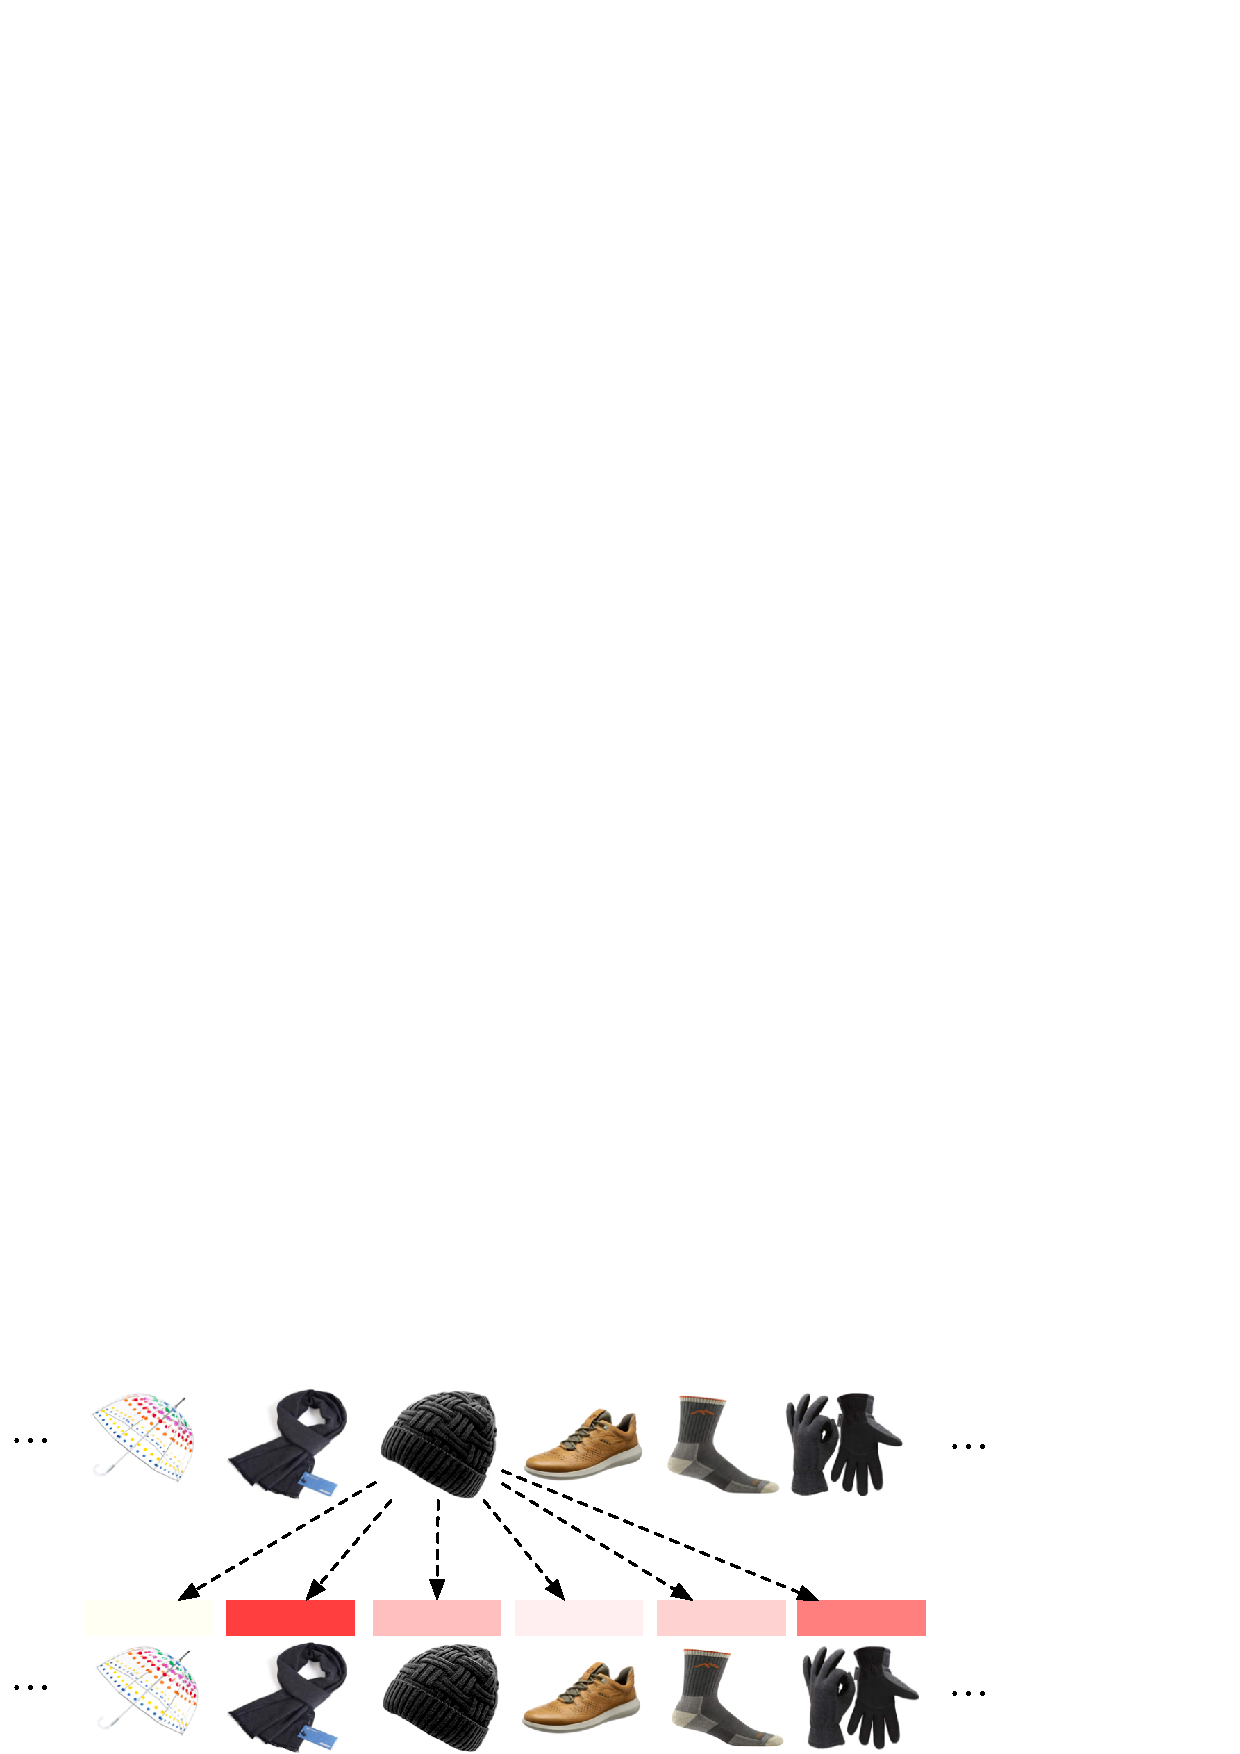
\includegraphics[width=1.0\columnwidth]{figure/attention.pdf}}
	\caption{Attention weight visualization. \textit{AtLocation} is required for prompt in the left column and \textit{PartOf} is required for prompt in the right column.} \label{fig:attention}
\end{figure}
Specifically, we focus on the attention weights between [MASK] token and 
other tokens in the prompt. A first glance of change of attention pattern 
is given in \figref{fig:LAMA} and we show more examples of other ConcetpNet 
relations in \figref{fig:attention}. We observe that while the original 
pretrained model tends to attend to special tokens like period and [SEP], 
the subnetwork successfully grasps the relevant concepts~(i.e., apple, 
worms, and basement) in the prompt hence produces the right object. 
We also use t-SNE~\citep{vanDerMaaten2008} to visualize the last layer's 
representation of [CLS] for each prompt. From \figref{fig:tsne}, the 
representations computed by original pretrained model are hardly separable as 
different types of knowledge are mixed together. In contrast, the pruned 
subnetwork can extract meaningful and disentangled representations for 
different commonsense relations.

\begin{figure}[th]
	\centering
	\scalebox{1.0}{\includegraphics[width=1.0\columnwidth]{figure/tsne_compare.pdf}}
	\caption{t-SNE visualization of [CLS]'s representation from original~(left) and pruned~(right) \textsc{BERT-base}.} \label{fig:tsne}
\end{figure}


\subsection{Commonsense Knowledge Base Completion~(CKBC)}
\label{sec:ckbc}
We evaluate the utility of identified relation-specific subnetworks on CKBC in an unsupervised manner. Specifically, we use the ConceptNet-100K benchmark provided by \citet{Li2016}. To ensure a fair evaluation, 
we manually create a subset of ConceptNet-100K 
consisting of triples with single-token subject/object. We also ensure that its dev/test set has \textbf{no overlap} with C-LAMA.
Each relation is associated with a sentence template~(provided in 
Appendix)~\citep{Kwon2019} of which the wording is distinct from 
those in C-LAMA. We acknowledge that these sentence templates might be suboptimal for certain relations, but prompt optimization is 
out of the scope of this paper. The resulting dataset contains 
$17,891$ training instances, $349$ development instances, 
and $446$ test instances.

\textbf{Link prediction.}~~We first formulate CKBC as a link prediction task 
and compare subnetworks~(i.e., $\mathcal{LM}_{\theta_r}$ 
is queried to predict missing link for instance of relation $r$) as well as original PLMs
against strong supervised KB completion mothods. 


\tabref{table:linkprediction} shows the results. Most of the supervised 
models outperform full-scale PLMs by a large margin, which suggests the 
inefficacy of directly using PLMs to perform link prediction. However, 
the subnetworks identified by our pruning procedure can
acquire performance on par with or better than state-of-the-art 
supervised models. Surprisingly, the pruned \textsc{DistilBERT} get the 
highest MRR, outperforming other larger and more advanced PLMs. 
\textsc{RoBERTa} struggles to predict correct objects, perhaps due to 
its larger vocabulary size compared to WordPiece~($50,265$ vs $30,522$) 
and less lexicon overlap~($53\%$ vs $59\%$) with the dataset.

%\KZ{It seems that our method (pruned models) don't work so well in the
%test set, compared to dev set. The scores for the same model between dev set and
%test set are also quite diff. Can you explain in this para?}

\textbf{Triple classification}~~We can also formulate CKBC as a triple classification task. Following ~\citet{Feldman2020}, we use estimated point-wise mutual information~(PMI) computed by pretrained language model as a surrogate of a triple's validity. An expectation-maximization-based Gaussian mixture clustering method is used and instances in the cluster with higher mean PMI are labeled as valid. 
\begin{table}[t]
	\centering
	\scriptsize
	\begin{tabular}{l|c}
		\toprule
		\textbf{Model} &  \textbf{F1 Score}\\
		\midrule
		\textsc{DistilBERT} & 74.1\\
		\textsc{DistilBERT}~(pruned) & \textbf{76.3}\\
		\midrule
		\textsc{BERT} & 73.7\\
		\textsc{BERT}~(pruned) & \textbf{76.7}\\
		\midrule
		\textsc{RoBERTa} &74.8 \\
		\textsc{RoBERTa}~(pruned) & \textbf{76.9}\\
		\midrule
		\textsc{MPNet} &76.5 \\
		\textsc{MPNet}~(pruned) & \textbf{78.0}\\
		\bottomrule
	\end{tabular}
	\caption{Triple classification on ConceptNet-100K.}
	\label{table:tripleclassification}
\end{table}
In our preliminary experiments, we found that the model pruned by the mask 
of a single relation might not be robust for PMI estimation and generally 
performed inferior to the intact model. 
In the same spirit as model ensembling, we then perform grid search over 
combinations of multiple knowledge, which is similar to what we did 
in zero-shot commonsense reasoning. For all four PLMs considered in 
\tabref{table:tripleclassification}, we observe that there exists one 
or multiple knowledge combinations delivering F1 score higher than the 
original models. 
%\KZ{Why is the difference between pruned and unpruned models
%not so big compared to link prediction?}

\textbf{Triple extraction.}~~We then investigate the ability of specialized 
subnetworks to extract novel commonsense knowledge triples absent 
from the dataset. We randomly sample 100 triples from the test set of 
ConceptNet-100K and for each sample use top-$K$ predictions from 
pruned \textsc{DistilBERT-base} as candidate objects. 
Three human annotators are asked to first determine the correctness of 
each candidate object and further determine their novelty~(i.e., not present 
in any of train/validation/test set) if deemed to be correct. 
The Fleiss Kappa inter-annotator agreement $\kappa$ is 0.66/0.65 
for precision and novelty, respectively.
\begin{figure}[t]
	\centering
	\scalebox{0.7}{\includegraphics[width=1.0\columnwidth]{figure/precision_novelty_2.pdf}}
	\caption{Precision-novelty curve with varied $K$.} \label{fig:extraction}
\end{figure}
\figref{fig:extraction} shows the change of precision-novelty with varied $K$. We observe a clear trade-off between the validity and novelty of triples extracted by the pruned model. As expected, a large $K$ inevitably makes noisy predictions but is more likely to extract unseen knowledge. For the purpose of knowledge enrichment, one might choose a large $K$ to ensure a desirable recall. We list the obtained novel triples in the Appendix D due to space limits.






\subsection{Commonsense Reasoning~(CSR)}
\label{sec:csr}
After identifying sparse subnetworks within PLMs that specialize in different commonsense knowledge, we now evaluate their generalization ability in the context of commonsense reasoning.
%One desirable outcome of our pruning procedure is the transformation from language representation to knowledge representation. We test if such subnetworks generalize in the context of commonsense reasoning.

\textbf{Many-shot learning.}~~We experiment with \textsc{BERT-base} and its deterministically pruned version using supervised fine-tuning on $7$ datasets: RTE~\citep{CambridgeJournals:6906264}, COPA~\citep{roemmele_choice_2011}, CommonsenseQA~\citep{talmor-etal-2019-commonsenseqa}, SWAG~\citep{zellers-etal-2018-swag}, HellaSWAG~\citep{DBLP:journals/corr/abs-1905-07830},   aNLI~\citep{DBLP:journals/corr/abs-1908-05739} and CosmosQA~\citep{huang-etal-2019-cosmos}. For each task, we identify the commonsense knowledge it might requires with a simple heuristic. Specifically, we obtain the five most frequent relations~(measured by how many times subject and object of certain relation appear in the context or answer) for each task and perform grid search over the combinations of these relationns. Then we take the union of masks for each relation and apply the resultant mask to the BERT as initialization for finetuning.
We repeat the training three times with different random seeds for each task. 
The  choice of mask combination for each task can be found in Appendix B.

The results in \tabref{table:finetuning} shows that, when initialized with proper weights, the model can be better fine-tuned on downstream commonsense reasoning tasks via more useful \textit{prior} knowledge. We further analyze the change of performance under the low-resource regime on COPA dataset. \figref{fig:copa} shows that the pruned \textsc{BERT} exhibits a notable advantage when training data is extremely scarce. As more training data is seen, the benefit of the pruned 
model becomes less prominent, i.e., $p>0.05$.
\begin{table}[t!]
	\centering
	\scriptsize
	\begin{tabular}{l|cc|c}
		\toprule
		\textbf{Task} & \textbf{Original} & \textbf{Pruned} &$p$-value \\
		\midrule
		RTE & 69.2$\pm${\scriptsize 2.3} & 69.8$\pm${\scriptsize2.0}& 0.12\\

		COPA & 62.4$\pm${\scriptsize 5.0} & 63.0$\pm${\scriptsize 4.7} &0.33  \\

		CommonsenseQA & 53.1$\pm${\scriptsize 0.6} & 54.1$\pm${\scriptsize 0.7} &0.08\\

		SWAG & 73.9$\pm${\scriptsize 0.3} & 74.2$\pm${\scriptsize 0.1} &0.09\\
		HellaSWAG & 38.9$\pm${\scriptsize 0.4} & 39.1$\pm${\scriptsize 0.5}&0.32  \\
		aNLI &63.7$\pm${\scriptsize 0.4} &64.0$\pm${\scriptsize 0.4}  &0.19\\
		CosmosQA &61.3$\pm${\scriptsize 1.0} &61.8$\pm${\scriptsize 0.2} &0.26\\
		\bottomrule
	\end{tabular}
	\caption{Finetuning results of \textsc{BERT} for CSR.}
	\label{table:finetuning}
\end{table}
\begin{figure}[t]
	\centering
	\scalebox{0.75}{\includegraphics[width=1.0\columnwidth]{figure/copa.pdf}}
	\caption{Finetuning result of \textsc{BERT} on COPA with varying portion of data.} \label{fig:copa}
\end{figure}
\begin{table*}[t!]
	\centering
	\scriptsize
	\begin{tabular}{l|cccccccc|c}
		\toprule
		\textbf{Model} &COPA-Tra. &COPA-Val. &CSQA &CA &WSC  &SM &ARCT1 &ARCT2 &Avg. \\
		\midrule
		\textsc{DistilBERT} &58.3 &60.0 &29.6 &84.6 &53.3  &71.6 &48.6 &50.4  &57.0  \\
		\textsc{DistilBERT}~(pruned) &\textbf{61.5} &\textbf{69.0} &\textbf{31.5} &\textbf{89.6} &\textbf{56.9}  &\textbf{72.1} &\textbf{53.4} &\textbf{51.6} & \textbf{60.7} \\
		\midrule
		\textsc{BERT} &60.2 &54.0 &26.5 &89.0 &57.3  &69.7 &46.8 &50.3 &56.7 \\
		\textsc{BERT}~(pruned) &\textbf{63.0} &\textbf{64.0} &\textbf{28.5} &\textbf{91.8} &\textbf{59.0}  &\textbf{71.7} &\textbf{50.0} &\textbf{52.0}  & \textbf{60.0}\\
		\midrule
		\textsc{RoBERTa} &60.7 &59.0 &39.9 &90.1 &61.8  &73.1 &48.6 &53.1 &60.7 \\
		\textsc{RoBERTa}~(pruned) &\textbf{65.3} &\textbf{72.0} &\textbf{40.4} &\textbf{93.4} &\textbf{62.9}  &\textbf{74.4} &\textbf{53.2} &\textbf{55.1} &\textbf{64.6}\\
		\midrule
		\textsc{MPNet} &66.5 &69.0 &40.0 &94.5 &64.3&75.8  &52.9 &56.7 &64.9  \\
		\textsc{MPNet}~(pruned) &\textbf{71.0} &\textbf{74.0} &\textbf{41.7} &\textbf{97.3} &\textbf{66.4}  &\textbf{77.5} &\textbf{56.1} &\textbf{57.7}  & \textbf{67.7}\\
		\bottomrule
	\end{tabular}
	\caption{Zero-shot results of accuracy~(\%) on commonsense reasoning tasks. Better results of each pair is in \textbf{bold}.}
	\label{table:zeroshot}
\end{table*}



\textbf{Zero-shot learning.}~~We next assess the ability of specialized 
subnetworks to perform zero-shot commonsense reasoning, a setting where 
the knowledge relied on to complete the task is solely determined by the model 
parameters. Here we focus on the following multiple-choice datasets: training set of COPA~(COPA-Tra.), validation set of COPA~(COPA-Val.), CommonsneseQA, Conjunction 
Acceptability~(CA)~\citep{Zhou2019}, 
Winograd Schema Challenge~(WSC)~\citep{levesque_winograd_2012}, 
SenseMaking~(SM)~\citep{wang-etal-2019-make}, 
ARCT1~\citep{habernal-etal-2018-argument} and 
ARCT2~\citep{DBLP:journals/corr/abs-1907-07355}. Each sample in the above datasets can be formulated as $\{[CLS]~context~[SEP]~choice_i ~[SEP]\}_{i=1}^{N}$, where $i$ is the subscript and $N$ is the number of choices. We compute the plausibility score of each choice using MLM head. Choice with the highest plausibility score is chosen as the answer. 

Since multiple types of knowledge are typically required for effectively 
reasoning over concepts, for each task, we perform grid search over 
combinations of $3$-$4$ different commonsense knowledge out of 
the $16$ total types and reported the best accuracy in \tabref{table:zeroshot}. 
We put the best combination for each model on each task in Appendix B
for space constraints. By combining multiple commonsense knowledge useful for the task, 
we show that the pruned models can actually surpass their full-scale 
version in all tasks considered in our experiments. 
The most likely explanation is that knowledge irrelevant to the specific task 
in the original models hurt the in-domain zero-shot reasoning capability. 
It also manifests that the most important reasoning skills vary from 
task to task.

\section{Discussion and Future Work}
\label{sec:discussion}
Our study has taken important initial steps in model 
evaluation and exploration by providing a lightweight yet 
effective method to reveal statistical biases and cues in NLU datasets. 
However, further exploration is needed to 
obtain a comprehensive understanding of model behavior.

First, as prompt impact varies across tasks and domains, 
future research will entail extensive prompt 
exploration and testing for specific applications.

Second, expanding our focus beyond the MNLI dataset's ``no''
feature to other features and tasks will help 
generalize our findings and deepen our 
understanding of prompt design and bias mitigation.

Third, the ``CoT'' strategy's effectiveness and generalizability 
in different settings and language models 
remain open questions, which we will address in future work.

By tackling these challenges, we aim to develop 
more reliable, robust, and unbiased AI systems 
through comprehensive model evaluation and bias mitigation research.


\section{Related Work}
\paragraph{Language models for phonetic reconstruction}
A related task of phonological ancient language reconstruction is proto-word reconstruction, which takes set of words in different contemporary languages as input and the corresponding word in their common ancestral language as result of supervised reconstruction. ~\citet{meloni_ab_2021} and~\citet{akavarapu_cognate_2023} both evaluate neural networks' performance on Romance language family's reconstruction task. ~\citet{kim_transformed_2023} first introduce Transformer architecture into proto-word reconstruction task and outperforms previous models on both Romance and Sinitic dataset. 
While large language models (LLMs) have recently demonstrated exceptional capabilities in understanding and generating contemporary languages, their proficiency in comprehending ancient Chinese, remains inadequate. \citet{zhang-li-2023-large}'s research highlights the limitations of LLMs in handling the complex ancient Chinese phonetic information.
\paragraph{Chinese phonetic dataset}
In terms of Chinese phonetic datasets, current digitization all organize the ancestor language (Middle Tang Chinese) and its daughter languages (modern Chinese dialects) into a cognate set. ~\citet{hou_j_xiandai_2004} first collecte 2,789 cognates of word-wise Chinese dialect pronunciation. ~\citet{chang_wikihan_2022} expand Hou's dataset, organize entries by characters instead of word.
As for chronological phonology dataset in Chinese, existing resources are mainly from studies of historical linguistics. Swedish sinologist Karlgren first put forward the phonological reconstruction of Middle Tang Chinese~\cite{TheReconstructionofAncientChinese}. ~\citet{wang_l_hanyu_2012} provides a comprehensive analysis of Chinese language phonological evolution. However, these sources are not digitized to our knowledge.
\section{Conclusion}
We implement a novel sequence-based dependency parsing
framework which takes advantage of high order features 
in parsing history. 
%We can also adapt beam search to this framework so as to
%relax the strictly greedy nature. Vine pruning\cite{rush2012vine} could
%be incorporated to speed up the parsing.
More importantly, we discovered that the parsing accuracy is very sensitive to
the quality of parsing sequence. Future work can be focused on
developing better sequence predictors that outperform Malt action classifier.
Furthermore, we use two sets of features for sequence predictor and
head mapper right now. A unified set of features between these two components
are worth exploring.
%Besides, better sequence predicting method and unified feature
%representation of two components are worth exploring.
%
%Though we currently get a not bad result,
%the sequence predictor still needs more exploration.
%According to our experiment, slightly changes
%on the sequence can lead to a fatal decline on accuracy. Ensuring the match degree of training sequence and testing
%sequence demands a high quality of sequence predictor.
%
%Further, the features in our current implementation are not expanded and well tuned yet  and we are free to define high order features to make use of parsing history. Our framework is flexible to merge other technics to enhance the performance. Introducing beam could make up for our greedy decoder and improve our accuracy. Vine pruning\cite{rush2012vine} could speed up parsing process. Besides, better sequence predicting method and unified feature representation of two components are worth exploring.

%\section*{Limitations}

In our study, there are some limitations that could be addressed in future research.
\begin{enumerate}
\item We currently only incorporate three mainstream psychotherapy approaches (i.e., PCT, CBT, SFBT) into Chain-of-Psychotherapies in this work, future explorations can include a wider range of psychotherapies like psychodynamics~\cite{Sheppard2006psychodynamics} to evaluate whether the more mixture, the better performance a chatbot will have.
\item  Despite our best efforts in designing the prompt for empathy analysis, the scores produced by GPT-4 are not highly accurate. Although GPT-4 is the most commonly employed model for assessing the generation effectiveness of LLMs~\cite{liu-etal-2023-g}, it tends to favor sentences generated by models like ChatGPT as higher quality, often deeming human responses as lower quality due to perceived inferior coherence compared to model-generated responses. Hence, it is imperative for us to explore more effective automated evaluation methods in the future.
\end{enumerate}
%\section{Ethical Statement}
In this work, we make every effort to minimize the risk of personal privacy leakage during the data collection process. We replaced usernames with random identifiers to prevent identification of users without external information. All datasets used in our study are either publicly available or adhere to their respective licenses. We sign and comply with the data use agreement to prevent privacy infringement or other potential misuses. All posts in examples were de-identified and paraphrased for anonymity.
What's more, we carefully considered the application of social media for the detection of mental illnesses. The purpose of this work is not to replace psychiatrists. Instead, we hope our model will be used as an effective auxiliary tool by experienced psychiatrists in the future.

\bibliography{refs}
%\def\year{2022}\relax
%File: formatting-instructions-latex-2022.tex
%release 2022.1
\documentclass[letterpaper]{article} % DO NOT CHANGE THIS
\usepackage{aaai22}  % DO NOT CHANGE THIS
\usepackage{times}  % DO NOT CHANGE THIS
\usepackage{helvet}  % DO NOT CHANGE THIS
\usepackage{courier}  % DO NOT CHANGE THIS
\usepackage[hyphens]{url}  % DO NOT CHANGE THIS
\usepackage{graphicx} % DO NOT CHANGE THIS
\urlstyle{rm} % DO NOT CHANGE THIS
\def\UrlFont{\rm}  % DO NOT CHANGE THIS
\usepackage{natbib}  % DO NOT CHANGE THIS AND DO NOT ADD ANY OPTIONS TO IT
\usepackage{caption} % DO NOT CHANGE THIS AND DO NOT ADD ANY OPTIONS TO IT
\DeclareCaptionStyle{ruled}{labelfont=normalfont,labelsep=colon,strut=off} % DO NOT CHANGE THIS
\frenchspacing  % DO NOT CHANGE THIS
\setlength{\pdfpagewidth}{8.5in}  % DO NOT CHANGE THIS
\setlength{\pdfpageheight}{11in}  % DO NOT CHANGE THIS
%
% These are recommended to typeset algorithms but not required. See the subsubsection on algorithms. Remove them if you don't have algorithms in your paper.
\usepackage{algorithm}
\usepackage{algorithmic}

\usepackage{graphicx, caption, subcaption}
\usepackage{amsmath}
\usepackage{color}
\usepackage{multirow}
\usepackage{booktabs}
\usepackage{bbm}
\usepackage{enumitem}
\usepackage[flushleft]{threeparttable}
\usepackage{makecell}
% \usepackage{hyperref}
\usepackage{amsfonts}
\usepackage[normalem]{ulem}
\newcommand{\KZ}[1]{\textcolor{blue}{Kenny: #1}}
\newcommand{\cut}[1]{}
%
% These are are recommended to typeset listings but not required. See the subsubsection on listing. Remove this block if you don't have listings in your paper.
\usepackage{newfloat}
\usepackage{listings}
\lstset{%
	basicstyle={\footnotesize\ttfamily},% footnotesize acceptable for monospace
	numbers=left,numberstyle=\footnotesize,xleftmargin=2em,% show line numbers, remove this entire line if you don't want the numbers.
	aboveskip=0pt,belowskip=0pt,%
	showstringspaces=false,tabsize=2,breaklines=true}
\floatstyle{ruled}
\newfloat{listing}{tb}{lst}{}
\floatname{listing}{Listing}
%
%\nocopyright
%
% PDF Info Is REQUIRED.
% For /Title, write your title in Mixed Case.
% Don't use accents or commands. Retain the parentheses.
% For /Author, add all authors within the parentheses,
% separated by commas. No accents, special characters
% or commands are allowed.
% Keep the /TemplateVersion tag as is
\pdfinfo{
/Title (Product Categorization for Multiple Evolving Businesses)
/Author (AAAI Press Staff, Pater Patel Schneider, Sunil Issar, J. Scott Penberthy, George Ferguson, Hans Guesgen, Francisco Cruz, Marc Pujol-Gonzalez)
/TemplateVersion (2022.1)
}

% DISALLOWED PACKAGES
% \usepackage{authblk} -- This package is specifically forbidden
% \usepackage{balance} -- This package is specifically forbidden
% \usepackage{color (if used in text)
% \usepackage{CJK} -- This package is specifically forbidden
% \usepackage{float} -- This package is specifically forbidden
% \usepackage{flushend} -- This package is specifically forbidden
% \usepackage{fontenc} -- This package is specifically forbidden
% \usepackage{fullpage} -- This package is specifically forbidden
% \usepackage{geometry} -- This package is specifically forbidden
% \usepackage{grffile} -- This package is specifically forbidden
% \usepackage{hyperref} -- This package is specifically forbidden
% \usepackage{navigator} -- This package is specifically forbidden
% (or any other package that embeds links such as navigator or hyperref)
% \indentfirst} -- This package is specifically forbidden
% \layout} -- This package is specifically forbidden
% \multicol} -- This package is specifically forbidden
% \nameref} -- This package is specifically forbidden
% \usepackage{savetrees} -- This package is specifically forbidden
% \usepackage{setspace} -- This package is specifically forbidden
% \usepackage{stfloats} -- This package is specifically forbidden
% \usepackage{tabu} -- This package is specifically forbidden
% \usepackage{titlesec} -- This package is specifically forbidden
% \usepackage{tocbibind} -- This package is specifically forbidden
% \usepackage{ulem} -- This package is specifically forbidden
% \usepackage{wrapfig} -- This package is specifically forbidden
% DISALLOWED COMMANDS
% \nocopyright -- Your paper will not be published if you use this command
% \addtolength -- This command may not be used
% \balance -- This command may not be used
% \baselinestretch -- Your paper will not be published if you use this command
% \clearpage -- No page breaks of any kind may be used for the final version of your paper
% \columnsep -- This command may not be used
% \newpage -- No page breaks of any kind may be used for the final version of your paper
% \pagebreak -- No page breaks of any kind may be used for the final version of your paperr
% \pagestyle -- This command may not be used
% \tiny -- This is not an acceptable font size.
% \vspace{- -- No negative value may be used in proximity of a caption, figure, table, section, subsection, subsubsection, or reference
% \vskip{- -- No negative value may be used to alter spacing above or below a caption, figure, table, section, subsection, subsubsection, or reference

\setcounter{secnumdepth}{2} %May be changed to 1 or 2 if section numbers are desired.

% The file aaai22.sty is the style file for AAAI Press
% proceedings, working notes, and technical reports.
%

% Title

% Your title must be in mixed case, not sentence case.
% That means all verbs (including short verbs like be, is, using,and go),
% nouns, adverbs, adjectives should be capitalized, including both words in hyphenated terms, while
% articles, conjunctions, and prepositions are lower case unless they
% directly follow a colon or long dash
\title{Enhanced Semantic Space: Integrate Concepts \\to Unify Dynamic Multi-Domain Product Categorization}
\author{
    %Authors
    % All authors must be in the same font size and format.
    % Written by AAAI Press Staff\textsuperscript{\rm 1}\thanks{With help from the AAAI Publications Committee.}\\
    Submission ID: 8044
    % AAAI Style Contributions by Pater Patel Schneider,
    % Sunil Issar,\\
    % J. Scott Penberthy,
    % George Ferguson,
    % Hans Guesgen,
    % Francisco Cruz\equalcontrib,
    % Marc Pujol-Gonzalez\equalcontrib
}
% \affiliations{
%     %Afiliations
%     \textsuperscript{\rm 1}Association for the Advancement of Artificial Intelligence\\
%     % If you have multiple authors and multiple affiliations
%     % use superscripts in text and roman font to identify them.
%     % For example,

%     % Sunil Issar, \textsuperscript{\rm 2}
%     % J. Scott Penberthy, \textsuperscript{\rm 3}
%     % George Ferguson,\textsuperscript{\rm 4}
%     % Hans Guesgen, \textsuperscript{\rm 5}.
%     % Note that the comma should be placed BEFORE the superscript for optimum readability

%     2275 East Bayshore Road, Suite 160\\
%     Palo Alto, California 94303\\
%     % email address must be in roman text type, not monospace or sans serif
%     publications22@aaai.org
% %
% % See more examples next
% }

% %Example, Single Author, ->> remove \iffalse,\fi and place them surrounding AAAI title to use it
% \iffalse
% \title{My Publication Title --- Single Author}
% \author {
%     Author Name
% }
% \affiliations{
%     Affiliation\\
%     Affiliation Line 2\\
%     name@example.com
% }
% \fi

% \iffalse
% %Example, Multiple Authors, ->> remove \iffalse,\fi and place them surrounding AAAI title to use it
% \title{My Publication Title --- Multiple Authors}
% \author {
%     % Authors
%     First Author Name,\textsuperscript{\rm 1}
%     Second Author Name, \textsuperscript{\rm 2}
%     Third Author Name \textsuperscript{\rm 1}
% }
% \affiliations {
%     % Affiliations
%     \textsuperscript{\rm 1} Affiliation 1\\
%     \textsuperscript{\rm 2} Affiliation 2\\
%     firstAuthor@affiliation1.com, secondAuthor@affilation2.com, thirdAuthor@affiliation1.com
% }
% \fi


% REMOVE THIS: bibentry
% This is only needed to show inline citations in the guidelines document. You should not need it and can safely delete it.
\usepackage{bibentry}
% END REMOVE bibentry

\newcommand{\TODO}[1]{\textcolor{red}{(todo: #1)}}
\newcommand{\secref}[1]{Section \ref{#1}}
\newcommand{\figref}[1]{Figure \ref{#1}}
\newcommand{\eqnref}[1]{Eq. (\ref{#1})}
\newcommand{\tabref}[1]{Table \ref{#1}}
\newcommand{\exref}[1]{Example \ref{#1}}
\newcommand{\tabincell}[2]{\begin{tabular}{@{}#1@{}}#2\end{tabular}}

\begin{document}

\maketitle

\begin{abstract}
    Product categorization is to assign a product with a suitable category, which is usually organized in a predefined taxonomy.
    As e-commerce platforms developing different business lines, a special but challenging categorization scenario emerges, where there are multiple domain-specific category taxonomies and each of them evolves dynamically over time. 
    In order to unify the categorization process and jointly utilize the cross-domain data, we propose a two-stage taxonomy-agnostic framework that relies solely on calculating the semantic relatedness 
    between product titles and category names in the vector space. 
    However, pure vector matching may fall for the surface form of text, 
    % \textbf{indulges the surface form of the text dominating the score model}, 
    and we thus further leverage the universal ``knowledge'' across different business domains to complement textual semantics.
    % to mitigate this issue. 
    We design a heuristic retrieval strategy and pretrain a contrastive ranking model with the help of ``concept'', which resembles the shared keyword knowledge cross domains. 
    % In the end, the semantic matching is the backbone of our framework, but the concept knowledge is the fuel to power the unified model. 
    Our comprehensive experiments show that our method outperforms existing sophisticated approaches quantitatively and efficiently on dynamical multi-domain taxonomies. 
\end{abstract}

\section{Introduction}

Protein$-$protein interactions (PPIs) are of central importance for the majority of biological functions, such as signal transduction, metabolic pathways, molecular dynamics, and protein networks\cite{Hoffmann.Krallinger.ea:2005}, for they serve as the most fundamental building blocks of the entire interacademic systems of any organisms. Collecting data on pairwise interaction relationships is essential for multiple purpose, including identification of modules with certain functionality\cite{Spirin.Mirny.03}, mapping diseases to dominated genes\cite{Ideker.Sharan.08}, and after all, understanding wholistic metabolic/genetic networks from a system biology perspective.

A lot of databases have been built to store protein and genetic interactions from major model organism species and are available in various standardized formats, such as MINT\cite{Zanzoni.Montecchi-Palazzi.ea:2002}, BIND\cite{Bader.ea:2003}, BIOGRID\cite{DBLP:journals/nar/StarkBRBBT06}, etc. Among those mainstream databases, the data largely rely on voluntary reports by scientists or researchers, besides, comprehensive curation efforts become indispensable for the sake of accuracy. However, the amount of biology-related literatures with respect to protein interactions grows explosively and thus make it either impossible or impractical to manually detect PPI information anymore.

Considering huge amount of PPI information with great wealth hidden in published papers, in recent years, numerous mining techniques have been proposed that aim to extract PPI information automatically from free text, especially machine learning, information retrieval, and natural language processing\cite{DBLP:journals/bib/WinnenburgWPDS08}.These approaches can be roughly categorized into three classes: co$-$occurrence, rule$-$based, and machine learning. 

Co$-$occurrence is the approach with most simplicity and naivete. Just as its name implies, this method intends to find out pairs of proteins that co-occur in the same context. The scope of "same context" ranges from phrase, sentence, paragraph to whole abstract, even document. The underlying assumption is that whenever two proteins are mentioned together by authors, chances are high that there is some kind of relationship between them. However, however, in-context closeness even semantic relation does not necessarily represent actual biological interaction. As a consequence, a large fraction of candidate pairs are mismatched inevitably, causing a high recall but low precision.

The second approach is rule-based extraction, in other words, pattern matching. There are many types of rules, most of them concern natural language processing (NLP). One way is to specify hand-crafted regular expressions before hand, which mostly lean on language usage preference. Besides, by using full or partial (shallow) parsing strategies, more information would be acquired, such as part-of-speech taggers, local dependencies between syntactic components, context-free grammar\cite{DBLP:journals/bioinformatics/TemkinG03}, and full sentence structure. Compared to co$-$occurrence, rule-based approach enjoy better precision but much lower recall. In addition, since the rules are usually derived from training data, that is to say, the improper choice of training data would be significantly lethal, therefore quality of extraction is invariably instable and may not applicable to other data.

The third and most commonly used approach use machine learning techniques, in this case, the task to extract protein$-$protein interactions turns out to be a binary classification problem. Each protein pairs are represented along with a set of features, which is associated with their context, then a well$-$defined classifier gives the answer whether the candidate protein pairs is classified to be qualified PPI. (TO BE FURTHER FILLED!!!)

In this paper, we introduce a general bootstrapping framework for Protein$-$protein interaction extraction from natural text.Our method differs from most of the previous works in three aspects:

(1)The extraction process is driven by only tiny fraction of training data, which are regarded as seed data. In each round, it would derive reliable patterns automatically from seed data, then extract more positive PPI pairs consequently, what's more, the seed data would be augmented by the newly extracted results with high confidence.

(2)multiple graph kernel. 

(3)various evaluation.




\section{Task Definition}
We formulate our recommendation problem as the sequential recommendation or next item prediction. Assume that each user $u$ has a corresponding interaction sequence $S_u$, which can be represented as \[S_u=\{(x_1,c_1,T_1),(x_2,c_2,T_2),...,(x_T,c_T,T_T)\},\] where $x_j$ denotes the $j$-th news articles that user $u$ interacts with, and $c_j$ denotes the context embedding vectors of the corresponding articles, and $T_j$ denotes the intra-session temporal information of the corresponding interactions. Noted that each user $u$ only appear once, $S_u$ is corresponding to different sessions. Each $S_u$ starts at time $T_u$.

The intra-session temporal information $T_j$ contains two part. One is the time of $j$-th interaction $Tc_j$, which means the time user $u$ \textit{clicks} the $j$-th article and reflects it's position in $S_u$. The other is the \textit{publish} time of $j$-th article $Tp_j$, reflecting the refreshness of it. The $T_u$ reflects the inter-session temporal information because sessions with close start time are more related to each other.

Given a target user $u$ with her sequential of interactive behaviors over items $S_u$, our personalized next-item recommendation task is to predict $x_{T+1}$ that the target user $u$ is most likely to access in his/her next visit. Noted that the long term history of user $u$ is invisible, and we're supposed to predict $x_{T+1}$ in real-time right away after sequential of interactive behaviors from $x_1$ to $x_T$. The whole procedure is depicted in \figref{fig:representation}.
\section{Approach}
%We first present our methods for testing short circuits in
%models, then modify some of these methods to create
%training data to reverse the short circuit problem
%and enhance the robustness of the models.
% 
%\subsection{Proxy Test for Short Circuit}
%We propose two types of approaches that can be used as proxy test for short circuits.
%One is through inspecting attention maps in
%the models under a white-box setting.
%The other is to generate new test cases by applying different operations on correct choices under a black-box setting.
%
%
%\subsubsection*{White-box Attention Weights~(AW)}
%One intuitive way to detect if an attention-based model is 
%exploiting short circuits is to visualize its attention map. 
%Given a well-trained model and a correctly answered MCQ  in the 
%form of \textit{[CLS] premise [SEP] choice [SEP]}, 
%where \textit{[CLS]} and \textit{[SEP]} are model-dependent 
%delimiters and \textit{choice} refers to the correct choice, 
%we first tokenize the input, feed the token sequence into the model, 
%and extract the attention map of all attention heads from the 
%last encoder layer.
%
%The attention maps are visualized through off-the-shelf tool~\cite{vig-2019-multiscale}
%into user-friendly demo as shown in \figref{fig:att-goodex}. 
%Human annotators are then asked to determine whether there exists 
%strong attention connections from the correct choice to the premise. 
%We consider the MCQ is solved without short-circuiting only if 
%over half of the annotators label it as having strong attention 
%connections. 
%
%Though accurate, such manual annotation is cost-prohibitive to be 
%scaled to larger tests. To remedy this issue, we propose 
%a rule-based procedure to automatically detect the short circuit 
%behavior of a model on MCQ. Specifically, we aggregate the 
%attention maps into one individual map by max-pooling over all 
%attention heads. Then we check if there exists at least one 
%attention score between token in the choice and token in the premise 
%higher than threshold $t_1$ or at least two higher than threshold 
%$t_2$, excluding special tokens like comma and period. 
%We consider that the model not short-circuiting on this MCQ if 
%neither of the two conditions is met. In practice, the 
%threshold $t_1$ and $t_2$ are tuned so as to maximally simulate 
%human annotation. The pseudo-code is shown in Algorithm \ref{AW}.
%
In this section, we first present our methods for testing short circuits in models, and then modify some of these methods to create training data to address the short circuit problem and enhance model robustness.

\subsection{Proxy Test for Short Circuit}
Since no existing method can definitively prove if a model is short-circuiting on a question, we propose two types of approaches that serve as proxy tests for short circuits. These approaches reveal the effects of model short-circuiting, though they can't directly prove the short-circuit itself, similar to dark matter. One approach involves inspecting attention maps in models under a white-box setting, while the other generates new test cases by applying different operations on correct choices under a black-box setting.

\subsubsection*{White-box Attention Weights~(AW)}

One intuitive way to detect if an attention-based model is exploiting short circuits is to visualize its attention map. Given a well-trained model and a correctly answered MCQ in the form of \textit{[CLS] premise [SEP] choice [SEP]}, where \textit{[CLS]} and \textit{[SEP]} are model-dependent delimiters and \textit{choice} refers to the correct choice, we first tokenize the input, feed the token sequence into the model, and extract the attention map of all attention heads from the last encoder layer.

The attention maps are visualized through an off-the-shelf tool~\cite{vig-2019-multiscale} into a user-friendly demo, as shown in \figref{fig:att-goodex}. Human annotators are then asked to determine whether there exists strong attention connections from the correct choice to the premise. We consider the MCQ to be solved without short-circuiting only if over half of the annotators label it as having strong attention connections.

Although accurate, such manual annotation is cost-prohibitive to be scaled to larger tests. To remedy this issue, we propose a rule-based procedure to automatically detect the short circuit behavior of a model on MCQ. Specifically, we aggregate the attention maps into one individual map by max-pooling over all attention heads. Then we check if there exists at least one attention score between a token in the choice and a token in the premise higher than threshold $t_1$, or at least two higher than threshold $t_2$, excluding special tokens like comma and period. We consider the model to not be short-circuiting on this MCQ if neither of the two conditions is met. In practice, the thresholds $t_1$ and $t_2$ are tuned to maximally simulate human annotation. The pseudo-code is shown in Algorithm \ref{AW}.


\begin{algorithm}
\small
	\caption{Attention Weight Thresholding}
	\label{AW}
\hspace*{0.02in} {\bf Input:} 
premise $P$, correct choice $C$, model $M$,  threshold $t_1$ and $t_2$. \\
\hspace*{0.02in} {\bf Output:}
binary 0/1 label $L$.
	\begin{algorithmic}[1]
		\State initialize counters $c_1$ and $c_2$ to 0.
		\State tokenize the formatted input as sequence of tokens $S$.
		\State feed $S$ into $M$ and extract the last layer's attention maps $Attn_{all}$.
		\State aggregate $Attn_{all}$ into $Attn_{max}$ by max-pooling over all attention heads.
		\For{$w_1$ in $C$}
		\For{$w_2$ in $P$}
		\If{$Attn_{max}(w_1, w_2)> t_1$}
				$c_1$ += 1
		\EndIf
		\If{$Attn_{max}(w_1, w_2) > t_2$}
				$c_2$ += 1
		\EndIf
		\EndFor
		\EndFor
		\State output 1 if $c_1>0$ or $c_2\geq 2$ and 0 otherwise.
	\end{algorithmic}
\end{algorithm}

\subsubsection*{Black-box Choice Operator}
\label{sec:proxy}
While attention-based testing methods can detect short circuits within the encoder directly, they don't directly detect short circuits in the end-to-end MCQ model, which also includes a linear layer above the attention-based pretrained language model. Additionally, these methods are limited to a family of models with inherent attention mechanisms.

A more desirable approach is an automatic end-to-end black-box test that is model-independent. In black-box testing, if a model correctly answers an MCQ, we slightly modify the MCQ by applying a certain``operation'' on the original correct choice to produce another wrong choice. The newly generated MCQ must share the same correct choice as the original question. By observing the model's response to the second MCQ, we can infer whether the model short-circuits on the original MCQ.If the model still selects the correct choice, then we consider it to have passed the test and not short-circuited on the original MCQ. The challenge now is how to construct the new wrong choice by implementing the operation in various ways.

In this paper, we consider the operations listed in \tabref{table:proxyop}. Some of the operations were mentioned in previous literature, while others are proposed here (marked with *).
The first line in each cell describes the operation, and the next two lines provide an example of constructing a false choice from a choice in the original question. An operation may either preserve (p) the truth value (\crosssymbol $\rightarrow$ \crosssymbol) or change (c) the truth value of the choice (\checksymbol $\rightarrow$ \crosssymbol).

\begin{table}[th]
        \centering
        \scriptsize
        \begin{tabular}{l|l}
                \toprule
                \textbf{Oper.} &\textbf{Description and Example}\\
                \hline
                \multirow{3}{*}{Neg+} & Add negation (c) \\
                & \textit{They called the police to come to my house. \checksymbol} \\
                & \textit{They {\color{olive}{didn't}}  called the police to come to my house. \crosssymbol} \\
                \hline
                \multirow{3}{*}{Neg-} &Remove negation (c) \\
                & \textit{Ben {\color{olive} never} starts working out. \checksymbol} \\
                & \textit{Ben starts working out. \crosssymbol}\\
                \hline

                \multirow{3}{*}{NER} &Randomly replace person names (c)\\
                 & \textit{A big wave knocked {\color{olive} Mary} down . \checksymbol} \\
                & \textit{A big wave knocked {\color{olive} Kia} down . \crosssymbol} \\
                \hline
                \multirow{3}{*}{PR*} & Switch pronoun by gender or quantity (c)\\
        &\textit{{\color{olive} She} had a great time .\checksymbol} \\
        &\textit{{\color{olive} He} had a great time . \crosssymbol} \\
                \hline
                \multirow{3}{*}{PI*} &Instantiate pronoun by randome person (c) \\
        &\textit{{\color{olive} They} gave Tom a new latte with less ice . \checksymbol}\\
        &\textit{{\color{olive} Nathanael} gave Tom a new latte with less ice . \crosssymbol}\\
                \bottomrule
%               \hline
                \multirow{3}{*}{Adv} &Add adverbs for emphasis (c) \\
                &\textit{The ocean was a calm as a bathtub .\crosssymbol} \\
                &\textit{{\color{olive} In fact} the ocean was a calm as a bathtub .\crosssymbol} \\
                \hline
               \multirow{3}{*}{CO*} & Crossover: Swap the true choices between two questions (p)\\ 
	&\textit{\color{olive}Josh got sick . \checksymbol} \\
	&\textit{\color{olive}{She had a great time .\crosssymbol}}  \\
\hline
                \multirow{3}{*}{Syn} &Replace adj/adv with synonym (p) \\
                &\textit{Dawn felt {\color{olive} happy} about getting away with it . \crosssymbol} \\
                &\textit{Dawn felt {\color{olive} glad} about getting away with it . \crosssymbol} \\

		\bottomrule
               \multirow{3}{*}{MT*} & Mutate: Swap two consecutive words (c) \\
		& \textit{Deb said yes {\color{olive} to} {\color{olive} Tim} 's marriage proposal. \crosssymbol} \\
		& \textit{Deb said yes {\color{olive} Tim} {\color{olive} to} 's marriage proposal .\crosssymbol} \\
               \hline
\multirow{3}{*}{Voice} &Swap subject and object (c) \\
        & \textit{{\color{olive}{Kara}} asked {\color{olive}{the neighbors}}  not to litter in their yard . \checksymbol} \\
        &\textit{{\color{olive}{the neighbors}} asked  {\color{olive}{Kara}}  not to litter in their yard . \crosssymbol}\\
                \bottomrule
        \end{tabular}
        \caption{A number of operations considered for proxy testing. 
First line in each cell describes the operation, the next two lines
give an example of how to construct a false choice from a choice of
the original question. An operation may either 
preserve (p) the truth value (\checksymbol $\rightarrow$ \checksymbol, \crosssymbol $\rightarrow$ \crosssymbol) or change (c) the truth value of
the choice (\checksymbol $\rightarrow$ \crosssymbol).  }
        \label{table:proxyop}
\end{table}

Inspired by boundary testing in software engineering, we can classify these operations into three equivalent classes (three vertical sections in \tabref{table:proxyop}), depending on the nature of the \textit{false} choice constructed:
\begin{enumerate}
\item The syntax and semantics are correct, and the \textit{false} choice appears similar to the \textit{true} choice.
\item The syntax and semantics are correct, and the \textit{false} choice appears distinct from the \textit{true} choice.
\item Either syntax or semantics is incorrect.
\end{enumerate}

The last class is not suitable for testing short circuits because the model may answer the proxy question correctly by eliminating the false choice due to errors in it, not by considering the premise.

We focus on perturbations on negation~\cite{checklist2020acl}, NER~\cite{checklist2020acl}, and pronouns in the first class and adverbial~\cite{wsp2020acl}, crossover, and synonym~\cite{checklist2020acl,wsp2020acl} in the second class.

While most of the operations are self-explanatory, the \textit{crossover} operation is unique and deserves special attention. Inspired by molecular biology, for each MCQ in the dataset that the model answers correctly, we substitute the original false choice with the true choice from another randomly sampled MCQ. The substituted choice remains false in the proxy question. The operation can be visually explained in \figref{fig:cross}.

\begin{figure}[th]
\centering
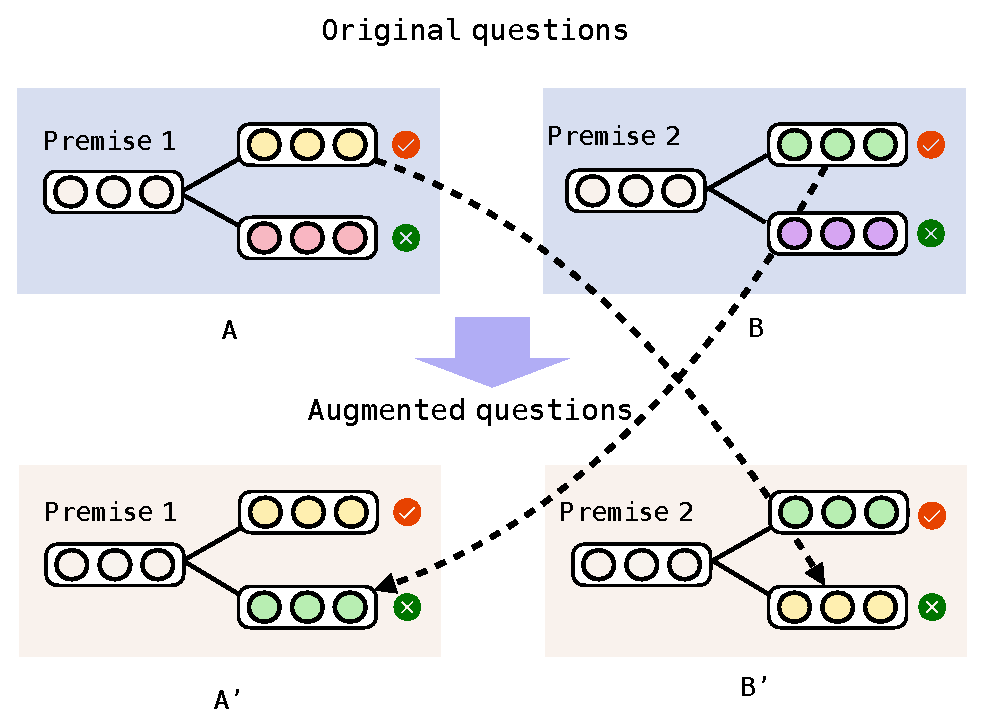
\includegraphics[width=\columnwidth]{figure/cross.eps}
\caption{The Crossover Operation: the true choice of both questions
are used to replace the false choices of these questions to create
two new proxy questions.}
\label{fig:cross}
\end{figure}

Compared to all other operations in classes 1 and 2, the crossover provides a proxy question that is most different from the original one but easier from a human perspective. This is because the two choices may be quite unrelated. If the model does not handle it correctly, it may be more indicative of a short circuit. As a result, the crossover is potentially a better short circuit test than others.

Another advantage of the crossover operation is that we can generate multiple false choices for an original question at a low cost, allowing us to test each original question more thoroughly. In contrast, most other operations cannot produce an adequate number of different variants of the original choice.

In summary, the proposed black-box choice operator provides a more generalizable and model-independent method for detecting short circuits in MCQ models. By applying various operations to create proxy questions, we can assess the model's performance and robustness more accurately, contributing to the development of better and more reliable models in the future.

\subsection{Improving Model Robustness by Data Augmentation}

If a model is shown to short-circuit by the proxy tests, its performance may decline, especially when applied to out-of-domain test data. To make models more robust, one natural thought is to generate more data to encourage models to focus on the relation between the premise and choices. While the operations used to generate proxy tests can also be utilized for data augmentation, not all of them are scalable or able to generate enough data for training.

The two operations that can generate a substantial amount of data are crossover and mutation. These operations can be applied to the training data to enhance the model's robustness.

\subsubsection*{Crossover for Data Augmentation}

Crossover is a good option for data augmentation because the two choices were originally true answers in their respective questions and presumably carry spurious features if the model was short-circuiting. By incorporating crossover into the training data, the model is forced to consider the premise in order to determine which choice is better.

\subsubsection*{Mutation for Data Augmentation}

Mutation has two flavors: (1) swap the words only in the true choice; (2) swap the words both in the true and the false choice. Compared to crossover, mutation has the potential to be more effective at improving model robustness. It not only forces the model to look into the premise due to its two very similar choices (same set of tokens), but also makes the model more sensitive to fine differences in word orders and enhances the model's prior grammatical knowledge.

\subsubsection*{Differentiating between Proxy Test and Data Augmentation}

It is essential to differentiate between the use of crossover and mutation operations in proxy tests and data augmentation. In proxy tests, these operations are used to modify the test data to assess the model's short-circuiting behavior. In contrast, when applied for data augmentation, the same operations work on the training data to enhance the model's robustness and generalization capabilities.

In conclusion, data augmentation through crossover and mutation operations can contribute to improving model robustness by encouraging models to focus on the relationship between the premise and choices. By incorporating these operations into the training data, models are forced to consider the premise and become more sensitive to the fine differences in word orders, leading to better performance and reliability in real-world applications.

\section{Experiments}
In this section, 
% after introducing the datasets we construct from multiple business lines, 
% we discuss our experimental results under single- \& multi-domain product categorization scenarios. A brief comparison of time efficiency between $\mathsf{TaLR}$ and simple \textit{Reranking} is also included. We also discuss the generalizability of $\mathsf{TaLR}$ under zero-shot conditions (evolving taxonomy  \& new taxonomy). 
we discuss experimental results under static multi-domain settings and dynamic (taxonomy evolving \& new taxonomy) conditions. A brief comparison of time efficiency between $\mathsf{TaLR}$ and simple \textit{Reranking} is also included.

% \subsection{Dataset Analysis}

\subsection{Baselines}
\label{sec: baseline}
% \TODO{Intro: TF-IDF+LR, fastText, BERT, multi-task,...}
We implement several baseline methods based on single-domain, multi-domain, and dynamic scenarios. 
To ensure fair comparisons, we also experiment concatenating product titles with meta concept text as input for some competitive baselines.
% \subsubsection{Single-domain}
% For methods targeting single-domain categorization tasks, we train individual models for each business. 
% As a system to be deployed in production environment with limited resources, 
Note that all the strong baselines are practicable in our online production environment, and those with unbearable space or time complexity are not considered. 
% We only choose practicable baselines that meet our production environment and 
Works holding different assumptions (e.g. necessitate multi-label or not support Chinese) with us are not considered either. 
Finally, we deploy and benchmark the following common baselines: 

\textit{Flat Classifier} \textbf{TF-IDF\&LR} represents product titles with TF-IDF weighted dense vectors, and executes classification with Logistic Regression. \textbf{FastText} \cite{bojanowski2017enriching} is a common baseline adopted in online product categorization challenges. 
% We also utilize pretrained 
\textbf{BERT} classifier is used as the strong baseline in both single-domain and multi-domain (trained with multi-task learning) settings.

\textit{Hierarchical Classifier} \textbf{HMCN}~\cite{wehrmann2018hierarchical} and \textbf{HiMatch}~\cite{chen2021hierarchy} leverage hierarchical information from taxonomy to 
guide the classification process, and we use BERT as a text encoder in both approaches. 
\textbf{XR-Linear} and \textbf{XR-Transformer} are two derivatives of PECOS~\cite{yu2020pecos} framework for extreme classification, which achieve competitive performance in most open product categorization datasets.

% HiMatch implicitly models hierarchical knowledge via GCN and positive \& negative node sampling.

% \subsubsection{Multi-domain}
% We exploit \textbf{multi-task} learning paradigm as strong baseline for multi-domain categorization. 
% % A shared BERT is utilized as the text encoder with multiple output heads targeting different tasks. 
% Data batches from each task take turns to update the model weights during training, and the loss function is formulated by summing up multi-class cross-entropy losses across different tasks.
% \subsubsection{Zero-shot Setting}
% \textit{Zero-shot Classifier} Since all the above baselines cannot tackle taxonomy evolving issues
% % (evolving taxonomy  \& new taxonomy) 
% without re-training, we adopt the vanilla BERT to encode both product titles and category names and calculate their [$\mathtt{CLS}$] similarity as a naive baseline \textbf{BERT-matching}. We further utilize separate BERT classifiers trained with few-shot data (1\%) on each task respectively as a strong baseline \textbf{BERT-few-shot}. \TODO{delete and move to each sub section}
% While each component of $\mathsf{TaLR}$ could be used individually under zero-shot scenarios, the ablations of $\mathsf{TaLR}$ can also be regarded as competitive zero-shot alternatives. 

\subsection{Experimental Setup}
We mix up training data from three datasets to train the unified $\mathsf{TaLR}$. 
We use \textbf{accuracy} score as the evaluation metric to meet real-world business demands.
Accuracy mathematically equals to \textbf{Micro-F1} score in a single-label multi-class classification problem. More details can be found in Appendix~\ref{appdix:exp detail}.

\subsection{Overall Results}
\label{sec:all res}

\begin{table}[!th]
\small
\setlength{\tabcolsep}{3.5pt}
  \begin{threeparttable}[b]
  \caption{The accuracy of baselines and our $\mathsf{TaLR}$ framework with variants on static multi-domain datasets. The best results are \textbf{bolded}, and the best baseline results are starred. Overall accuracy is the weighted average w.r.t respective test set size. $\mathsf{MS}$: mapping scorer, $\mathsf{CL}$: contrastive learning. 
  % ``+concept'' means concatenation of concepts after the product title, and (-) means ablation. 
  % \xiujie{(+) ... ablation?}
  }
  \label{tb:all}
  \centering
  \begin{tabular}{l|llll}
    \toprule
    Methods & Overall & \multicolumn{1}{c}{QD} & \multicolumn{1}{l}{\;BH} & \multicolumn{1}{l}{\;FG}\\
    \midrule
    \multicolumn{5}{c}{Separate models}\\
    \midrule
    TF-IDF\&LR $ $ & 69.51 & 69.93 & 68.23 & 69.95 \\
    FastText $ $ & 74.62 & 74.01 & 71.68 & 80.82 \\
    BERT $ $ & 83.49 & 84.82 & 79.93$^*$ & 84.23\\
    BERT+$\spadesuit$  $ $ & 83.01 & 86.45 & 79.02 & 75.32\\
    % HFGN-F-classifier $ $ & - & 83.72 & 77.09 & 84.25 \\
    HMCN-F-BERT $ $ & 82.14 & 83.72 & 77.09 & 84.25 \\
    HiMatch-BERT $ $ & 84.08 & 86.12 & 77.38 & 84.19 \\
    HiMatch-BERT+$\spadesuit$$ $ & 83.75 & 87.26$^*$ & 77.26 & 78.53 \\
    XR-Linear$ $ & 76.57& 75.27 & 77.91 & 78.95 \\
    XR-Transformer$ $ & 84.58$^*$ & 79.74 & 79.23 & 84.58$^*$ \\
    XR-Transformer+$\spadesuit$$ $ & 81.45 & 85.34 & 74.59 & 78.53  \\
    \midrule
    (a): $\mathsf{TaLR}$ $ $ & 85.90 & 87.88 & 81.92 & 85.09\\
    \midrule
    \multicolumn{5}{c}{Unified model}\\
    \midrule
    % BERT Multi-task & 64.41 & 76.79 & 50.26 & 44.09 \\
    BERT Multi-task & 68.00 & 80.27 & 50.28 & 44.29 \\
    BERT Multi-task+$\spadesuit$ & 67.79 & 81.37 & 49.77 & 39.83 \\
    (b): $\mathsf{TaLR}$ & \textbf{86.23} & \textbf{88.16} & \textbf{82.48} & \textbf{85.25}\\
    \midrule
    \multicolumn{5}{c}{$\mathsf{TaLR}$ ablation test}\\
    \midrule
    % (-) rerank stage & {82.29}  & 84.19  & {77.63}  & 82.72 \\
    % (-) retrieval stage & 83.29  & 84.95  & 80.53  & {81.78} \\
    % \midrule
    % \midrule
    (c): (b) (-) $\mathsf{CL}$ & 85.26  & 86.83  & 81.75  & 85.13 \\
    (d): (b) (-) $\mathsf{MS}$ & {84.63}  & {86.59}  & {80.13}  & {84.71}  \\
    (e): (b) (-) $\mathsf{CL}$\&$\mathsf{MS}$ & 82.82 & 83.85 & 79.15 & 84.71 \\
    (f): (b) (-) $\mathsf{CL}$\&$\mathsf{MS}$ +$\spadesuit$ & 84.38 & 87.43 & 80.64 & 79.77 \\

    % (-) vector-based retrieve & 84.91  & 86.52  & 81.66  & 84.28  \\

    \bottomrule
  \end{tabular}
  \begin{tablenotes}
    % \item[1] The overall accuracy is the weighted average of results on three domains, where weights are determined by the size of their corresponding test set.
    % We list separate accuracy on each subset.
    % \item[2] Methods with $ $ notation train three separate models on the three datasets of business lines and infer using its corresponding model. Methods without $ $ only train one unified model using multi-domain data.
    % \item[3] (-) denotes the ablation of following modules in $\mathsf{TaLR}$.
    \item[$\spadesuit$] concatenate concept text after product title
    \item[(-)] ablate cretain modules
    % \item[$\mathsf{MS}$] mapping scorer module
    % \item[$\mathsf{CL}$] contrastive learning module
  \end{tablenotes}
  \end{threeparttable}
\end{table}
The overall accuracy score is shown in \tabref{tb:all}.
% , and we can make the following observations.
Since traditional single-domain approaches cannot tackle \textbf{multi-domain taxonomies}, we train \textbf{separate} models on each business respectively. 
Among methods targeting one static taxonomy, hierarchical classifiers generally perform better than flat classifiers
% mainly because it leverages 
with the aid of taxonomy structure information.
% utilizes the positive and negative relationship of nodes in taxonomy.
However, because these methods can only handle one static taxonomy, they not only suffer from efforts to maintain different models for each domain but also fail to leverage multi-domain data. 
While the multi-task BERT is able to train and infer on three domains within one model, it performs even worse than TF-IDF\&LR on BH and FG. 
One possible reason is that the multi-task approach relies heavily on the weighting of losses, and if the task-specific training data distribution varies significantly, one task might dominate the joint distribution and constrain the optimization of other tasks. 
% Straightforwardly 
Simply concatenating meta concepts to titles does not always take effect,
% for these methods on some domains, 
and this is expected since concatenated tokens implicitly contribute to the joint representation of one sentence (e.g. self-attention in transformer), which proves to be inferior to our explicit usage of statistical mapping and contrastive grouping.
% this is expected since short concept texts can not dominate the surface form of titles, and these methods does not optimize relatedness in a macroscopic view. \zelin{not clear}


For our proposed framework $\mathsf{TaLR}$, variant (a) already outperforms other baselines in separate model training paradigm, while $\mathsf{TaLR}$ (b) further achieves even higher accuracy when jointly trained on the mixed multi-domain data where the multi-task BERT fails,
verifying $\mathsf{TaLR}$'s efficacy on \textbf{multi-domain taxonomies}. 
% As is shown, the unified $\mathsf{TaLR}$ (b) is better than separate $\mathsf{TaLR}$ (a), and 
We assume that the measurement of semantic relatedness is transferable on either business domain, and their shared knowledge could be integrated via contrastive pretraining as well. 
% We assume that some products and category names from multiple domains 
% may share similar semantic meanings as well as concepts knowledge, 
Therefore, the unified training helps improving the performance on each respective domain instead of conflicting each other as BERT multi-task does. 
% This is our cross-domain \textbf{knowledge integration} assumption and is thus verified. 
% \zelin{not clear}
% \zelin{not perspicuous}
% Furthermore, when we compare $\mathsf{TaLR}$ (-) reranking (a single BERT bi-encoder) and $\mathsf{TaLR}$ (-) retrieval (a single BERT cross-encoder) with the BERT-classifier, the results is close. 
% This first elucidates that these two stages are reinforcing each other, and further corroborates that the improvement of $\mathsf{TaLR}$ from $\mathsf{TaLR}$ $ $ is contributed by the \textbf{knowledge integration} capability of the framework instead of purely addition of data.

From the ablation tests, we can observe the effectiveness of the two plug-in modules in our $\mathsf{TaLR}$ framework from row (c) and (d), and the contribution of these two modules are orthogonal. 
Removing the mapping scorer in (d) drops the overall accuracy most, 
while removing contrastive pretraining in (c) results in its inferior performance than (a) as well. 
This indicates both modules are indispensable for the enhancement of exploiting multi-domain data.
% Compared with (e)$\rightarrow$(c) and (e)$\rightarrow$(d), (e)$\rightarrow$(f) improves the least in overall accuracy, showing that our two plug-in modules are more effective than simply concatenation of concepts. 
From (e)$\rightarrow$(f), concatenating meta concepts somehow improves the overall performance, but (f) still loses to (b). This reaffirms our above assumption that our usage of meta concepts is superior to simple concatenation. 
% \zelin{no key point}
% showing that our model with concept grouping can semantically align the embeddings of product titles and category names from multiple domains. 
% Removing the concept retrieval unit impairs the overall results significantly, mainly on account of the external knowledge imported from the concept set. 
To further analyze the effects of the two plug-in modules, we conduct Case Study in Appendix~\ref{sec:appdix-case}.

\subsection{Time Consumption} 
\label{sec:time cons}
% A big concern of our framework is to limit the run-time overheads, since the large label space challenge may deteriorate in one-vs-all retrieval systems rather than classification approaches.  
To meet online deployment requirement, the inference time consumption (seconds cost for each instance) needs to be considered. We compare $\mathsf{TaLR}$ with the vanilla model (single BERT cross-encoder) on the three datasets in \figref{fig:time}.
% , and we train and test on our three standard datasets. 
% Here the single BERT cross-encoder computes the similarity score over all category classes and selects the most similar one as the prediction, while $\mathsf{TaLR}$ instead utilized bi-encoder with cached category embeddings to conduct one-vs-all retrieval and the cross-encoder BERT in \textit{Reranking} stage takes only 10 candidates. 
% \figref{fig:time} plots the relationship between the number of classes and the inference time. 
On the one hand, the inference speed of $\mathsf{TaLR}$ is much faster (4 times faster for FG and 10 times faster for BH) than vanilla model owing to the \textit{Retrieval} stage. On the other hand, the time consumption per item of $\mathsf{TaLR}$ increases almost linearly along with the number of classes, while for vanilla model the overhead grows more sharply, revealing the time efficiency of $\mathsf{TaLR}$ when the class number scales up. 
% As for the accuracy score, $\mathsf{TaLR}$ fluctuates in the same pace with BERT cross-encoder but consistently outperforms it, and the reason of fluctuation is explained before.
% $\mathsf{TaLR}$ also consistently outperforms single BERT cross-encoder in accuracy due to the selection of better candidates in \textit{Retrieval} stage. 

\begin{figure}[thbp] \centering
    \includegraphics[width=0.4\textwidth]{time.pdf}
    \caption{Accuracy results and inference time consumption when the number of classes grows.} 
    \label{fig:time}
\end{figure}

\subsection{Dynamic Test Set Experiment}
\label{sec:evolve res}
In order to evaluate the ability of our framework on \textbf{taxonomy evolving} challenge, 
we use $\mathsf{TaLR}$ trained on the original multi-domain datasets to directly infer on two dynamic test sets. The vanilla BERT without any finetuning is a naive baseline \textbf{BERT-matching}. The BERT fine-tuned with few-shot new data (1\%) is a strong baseline \textbf{BERT-few-shot}.
% we directly infer product titles with $\mathsf{TaLR}$ trained on multi-domain datasets on the evolved taxonomies.
% we conduct experiments to directly infer evolved new category of the product with $\mathsf{TaLR}$. 
Here ``before'' denotes the subset from the original test set and ``after'' denotes the subset with the same product titles but evolved categories.
From the listed accuracy ``before'' and ``after'' taxonomy evolving in \tabref{tb:evolve}, we can conclude that $\mathsf{TaLR}$ sustains satisfactory accuracy compared with its strong counterpart trained with 1\% extra data.
% the encoded [$\mathtt{CLS}$] token similarity from %%% explained before
% BERT-matching is the vanilla similarity matching baseline and BERT-few-shot is the separate few-shot classifiers we mentioned in \secref{sec: baseline}. Note that BERT-few-shot is trained on full data before evolving.

\begin{table}[th]
\small
\setlength{\tabcolsep}{1.8pt}
  \begin{threeparttable}[b]
  \caption{The accuracy on two dynamic test sets. $\Delta$ is the change
  of accuracy after evolving. The best ``after'' scores and least drop $\Delta$ are bolded.}
  \label{tb:evolve}
  \centering
  \begin{tabular}{l|ccc|ccc}
    \toprule
    \multirow{2}{*}{Methods} & \multicolumn{3}{c|}{QD$-divide$} & \multicolumn{3}{c}{QD$-integrate$}\\
    \cline{2-7}
    & Before & After & $\Delta$ & Before & After & $\Delta$ \\
    \midrule
    BERT-matching & 6.66 & 11.95 & \textbf{+5.29} & 13.39 & 2.23 & -11.16\\
    BERT-few-shot & 90.51 & 43.54 & -46.96 & 86.79 & 50.16 & -36.53\\
    \midrule
    $\mathsf{TaLR}$ & 90.11 & \textbf{69.71} & -20.40 & 85.20 & \textbf{81.48} & \textbf{-3.72}\\
    % (-) contrastive  & 89.10 & \textbf{79.21} & -9.89 & 84.11 & 80.02 & -4.09\\
    % (-) rerank stage & 89.70 & 73.94 & -15.76 & 86.36 & 81.47 & -4.89\\
    % (-) rule-based unit & 89.51 & 64.25 & -25.26 & 84.61 & 81.19 & \textbf{-3.42}\\
    \bottomrule
  \end{tabular}
%   \begin{tablenotes}
%     \item[1] 
%   \end{tablenotes}
  \end{threeparttable}
\end{table}
% {too long, rewrite}
% On the one hand, our $\mathsf{TaLR}$ even outperforms BERT-few-shot without additional training on evolved taxonomies, which indicates its robustness in handling dynamic issues.
% On the other hand, we can observe an opposite trend of BERT-matching and $\mathsf{TaLR}$ through $\Delta$ when two different evolving challenges are encountered. In the node $integrate$ scenarios, $\mathsf{TaLR}$ exhibits robustness with a slight drop of accuracy. 
% When progressively ablating contrastive learning and the whole \textit{Reranking} stage, the accuracy of $\mathsf{TaLR}$ consistently decreases, which indicates their contributions to the node \textit{integrate} variants in evolving taxonomy.
% % \textbf{Taxonomy integration}.
% % On the other hand, BERT-matching suffers from a drastic drop in accuracy, which may attribute to 
% However in the node $divide$ scenario, wherever contrastive learning is incorporated, there is a substantial drop in $\Delta$. Completely excluding the contrastive learning while keeping all other components gives the best accuracy. 
% The reason behind it is that contrastive learning tends to make the representations of products from the same category tied closer, while the division of nodes breaks this relation. 


\subsection{Extrapolating Results on New Taxonomy}
\label{sec:new tax}

% For multi-domain business lines, 
Consider an extreme \textbf{taxonomy evolving} condition when a new business line emerges, a robust model is supposed to categorize incoming products based on the brand-new taxonomy. 
% Hence it poses challenge for $\mathsf{TaLR}$ to zero-shot transfer to new domains so as to improve user experience in this cold-start scenario.

\begin{table}[th]
%   \begin{threeparttable}[b]
  \small
  \caption{The accuracy of $\mathsf{TaLR}$ on the new taxonomy. }
  \label{tb:zeroshot}
  \centering
  \begin{tabular}{l|ccc}
    \toprule
    Methods & QD & BH & FG \\
    \midrule
    BERT-matching & 9.00 & 11.23 & 4.03 \\
    BERT-few-shot & 43.29 & 35.19 & 29.80 \\
    % BERT-product & 52.00 & 48.81 & 51.32 \\
    \midrule
    $\mathsf{TaLR}$ & \textbf{60.57} & \textbf{65.45} & \textbf{62.69}\\
    % $\mathsf{TaLR}$-few(?) &  &  & \\
    % $\mathsf{TaLR}$-finetune(?) & 84.32 & 76.40 & 83.59\\
    % \midrule
    (-) contrastive & 56.71 & 64.99 & 60.79\\
    % (-) Rerank stage & 53.79 & 59.56 & 57.68 \\
    (-) mapping scorer & 56.25 & 64.65 & 59.29\\
    \bottomrule
  \end{tabular}
%   \begin{tablenotes}
%     \item[1] 
%   \end{tablenotes}
%   \end{threeparttable}
\end{table}

We deploy our experiments in a zero-shot manner, where we take turns to train $\mathsf{TaLR}$ on either two business data and test its performance on the remaining business. $\mathsf{TaLR}$ still outperforms BERT-few-shot. 
% We compare $TaLR$ with BERT-matching model and bi-encoder BERT in zero-shot, and $TaLR$-zero sustains better accuracy, 
% This indicates that $\mathsf{TaLR}$'s ability capturing semantic relatedness between product titles and category names on original domains could be seamlessly transferred to new domains with new taxonomies.
This shows $\mathsf{TaLR}$'s preeminent transferability with the reformulation of textual semantic matching, which helps improving user experience in this cold-start scenario.
% It mainly contributes to the learning in the other two domains, 
% which enhances the semantic relatedness understanding in the third dataset with brand new taxonomy.
Each component in the ablation test verifies its effectiveness as well. 

% More details about ablation setting is in \secref{sec:exp detail}.



% \subsection{Different Retrieval Strategies}
% \label{sec:retri stra}
% In \textit{Retrieval} stage, it is encouraged to exploit the potential candidates as accurately as possible, otherwise the latter \textit{Reranking} stage would never make right predictions if the true label is not covered by the retrieved candidates. Hence we use HR@$k$ to measure the retrieval performance.

% Firstly, we compare several alternatives of the loss function in vector-based retrieval model. In \figref{fig:vector-retri}, as $k$ goes on, the HR score increases, and the model trained with Cosent loss is consistently better than others, while the model trained with SBERT loss performs unstably, sometimes worse than Cosine loss. 
% One explanation is that comparing with Cosine loss and SBERT loss, the Cosent loss focuses on the positive-versus-negative pairwise optimization, which means the model only cares for the relative order of the prediction results instead of the specific value. And this setting brings consistent recall of candidates.
% \begin{table}[th]
%   \caption{The retrieval results of the vector-based unit over different loss function. The best results are bolded.}
%   \label{tb:vector-retrieval}
%   \centering
%   \begin{tabular}{c|c|ccc}
%     \toprule
%     Loss & Dataset & HR@1 & HR@5 & HR@10 \\
%     \midrule
%     \multirow{3}{*}{Cosine} & QD & 74.80 & 82.28 & 84.46\\
%     & BH & 72.75 & 81.77& 84.04\\
%     & FG & 65.59 & 80.40 & 83.23\\
%     \midrule
%     \multirow{3}{*}{SBERT} & QD & 82.25 & 88.96 & 90.92\\
%     & BH & 76.95 & 86.76 & 89.41\\
%     & FG & 80.67 & 87.27 & 88.86\\
%     \midrule
%     \multirow{3}{*}{Cosent} & QD & 84.19 & 88.97 & 90.30\\
%     & BH & 77.64 & 85.27 & 87.18\\
%     & FG & 82.72 & 86.66 & 87.48\\
%     \bottomrule
%   \end{tabular}
% \end{table}

% \begin{figure}
%   \begin{subfigure}[b]{0.49\columnwidth}
%   \centering
%   \includegraphics[width=\columnwidth]{hr_1.pdf}
%   \caption{HR@1}
%   \end{subfigure}
% %   \hfill
% %   \begin{subfigure}[b]{0.49\columnwidth}
% %   \centering
% %   \includegraphics[width=\columnwidth]{hr_5.pdf}
% %   \caption{HR@5}
% %   \end{subfigure}
%   \hfill
%   \begin{subfigure}[b]{0.49\columnwidth}
%   \centering
%   \includegraphics[width=\columnwidth]{hr_10.pdf}
%   \caption{HR@10}
%   \end{subfigure}
%   \caption{The retrieval results of the vector-based unit over different loss functions.}
%   \label{fig:vector-retri}
% \end{figure}

\cut{
To generate better candidates, we adopt several heuristic algorithms for two-way candidates fusion.
% the vector-based unit and rule-based unit. 
\tabref{tb:fusion} depicts the retrieval results over different fusion strategies. The size of merged candidate sets is not stuck to $10$ for some of the strategies, so we list the average number.
Generally, the \textbf{Rule-First} algorithm achieves better scores, and \textbf{De-Dupli} algorithm is competitive with it. We use \textbf{Rule-First} in our framework due to its fixed candidate size which is more convenient to process.
Although the pure vector-based unit performs less effectively than the rule-based counterpart, they could complement each other after fusing together with the help of an ensembled understanding of textual semantics and training set distribution.
% the ensemble of vector-based unit and rule-based unit strengthens the performance of rule-based unit, revealing that vector-based unit can better understand the instance semantically that rule-base unit can not. 
More discussions are in Case Study.

\begin{table}[th]
\setlength{\tabcolsep}{2pt}
  \caption{The retrieval results of candidates for different fusion strategies. The best results are bolded.}
  \label{tb:fusion}
  \centering
  \begin{tabular}{c|cc|cc|cc}
    \toprule
    \multirow{2}{*}{Strategy}  & \multicolumn{2}{c|}{QD} & \multicolumn{2}{c|}{BH} & \multicolumn{2}{c}{FG} \\
    \cline{2-7} 
      & Recall & Size & Recall & Size & Recall & Size \\
    \midrule
    Rule-based & 95.33 & 8.6 & 96.77 & 8.8 & 97.32 & 9.0 \\
    Vec-based & 90.30 & 10 & 87.18 & 10 & 87.48 & 10 \\
    \midrule
    De-Dupli & 96.08 & 10.5 & \textbf{97.54} & 10.4 & 97.77 & 10.7 \\
    Norm\&Rank & 93.74 & 10 & 92.42 & 10 & 92.77 & 10 \\
    Rule-First & \textbf{96.12} & 10 & 97.48 & 10 & \textbf{98.01} & 10 \\
    \bottomrule
  \end{tabular}
\end{table}
}
% \section{Case Study}
% For product ``\textit{red dancing shoes (size 35)}'', which should be categorized to \verb|Sports/Outdoors| $\rightarrow$ \verb|Yoga/Dancing| $\rightarrow$ \verb|Dancing Shoes|, the vector-based unit retrieves the correct class as top-$1$ answer, but the rule-base unit retrieves \verb|Clothes/Shoes| $\rightarrow$ \verb|Woman Shoes| $\rightarrow$ \verb|Woman Slippers| as top-$1$. This time the distribution knowledge guides the rule-based model towards a wrong direction, while the vector-based model succeeds relying on the semantic similarity.

% For product ``\textit{CHEERS$^\circledR$ 12 years}'', the vector-based model categorizes it to \verb|Books| $\rightarrow$ \verb|Economics/Management| $\rightarrow$ \verb|Marketing|, whereas the rule-based unit correctly retrieves \verb|Alcoholic Drinks| $\rightarrow$ \verb|Imported Liquors| $\rightarrow$ \verb|Whisky|. This shows that ``12 years'' misleads the vector-based model to the semantic meaning of economics, and rule-based unit successfully leverages its distribution knowledge in training set.

% For product ``\textit{towel gourd\&soy bean (towel gourd 1 pcs, soy bean 150g)}'', both rule-based unit and vector-based unit predict
% \verb|Vegetable| $\rightarrow$ \verb|Soy Product| $\rightarrow$ \verb|Soy Bean| wrongly as top-$1$, whereas $\mathsf{TaLR}$ classifies it to correct \verb|Vegetable| $\rightarrow$ \verb|Mixed Product| $\rightarrow$ \texttt{Vegetables mixture}, and clearly, the contribution is from the following \textit{Reranking} stage.
% \begin{table*}[t]
%   \caption{The retrieval results of candidates for different fusion strategies. The best results are bolded.}
%   \label{tb:fusion}
%   \centering
%   \begin{tabular}{c|c}
%     \toprule
%     Product title & \textit{red dancing shoes (size 35)} \\
%     \midrule
%     Ground truth & \verb|Sports/Outdoors| $\rightarrow$ \verb|Yoga/Dancing| $\rightarrow$ \verb|Dancing Shoes| \\
%     Vector-based top-$1$ & \verb|Sports/Outdoors| $\rightarrow$ \verb|Yoga/Dancing| $\rightarrow$ \verb|Dancing Shoes| \\
%     Rule-based top-$1$ & \verb|Clothes/Shoes| $\rightarrow$ \verb|Woman Shoes| $\rightarrow$ \verb|Woman Slippers| \\
%     \midrule
%     Product title & \textit{CHEERS$^\circledR$ 12 years} \\
%     \midrule
%     Ground truth & \verb|Alcoholic Drinks| $\rightarrow$ \verb|Imported Liquors| $\rightarrow$ \verb|Whisky| \\
%     Vector-based top-$1$ & \verb|Books| $\rightarrow$ \verb|Economics/Management| $\rightarrow$ \verb|Marketing| \\
%     Rule-based top-$1$ & \verb|Alcoholic Drinks| $\rightarrow$ \verb|Imported Liquors| $\rightarrow$ \verb|Whisky| \\
%     \midrule
%     Product title & \textit{towel gourd \& soy bean (towel gourd 1 pcs, soy bean ~150g)} \\
%     \midrule
%     Ground truth & \verb|Vegetable&/ Product| $\rightarrow$ \verb|Mixed Product| $\rightarrow$ \verb|Vegetables mixture| \\
%     Vector-based top-$1$ & \verb|Vegetable/&Soy Product| $\rightarrow$ \verb|Soy Product| $\rightarrow$ \verb|Soy Bean| \\
%     Rule-based top-$1$ & \verb|Vegetable/Soy Product| $\rightarrow$ \verb|Soy Product| $\rightarrow$ \verb|Soy Bean| \\
%     \bottomrule
%   \end{tabular}
% \end{table*}



\subsection{Online Experiment}
% We conduct online experiments on one downstream task where the category of a product is needed, 
% % of semantic vector space, 
% that is the main page recommendation (multi-domain). 
% % After deploying our contrastive pretrained model to compute the hidden vector representations of related products and utilizing this in sophisticated 
% When $\mathsf{TaLR}$ is incorporated in the
% recommendation system, customer purchase click rate increases significantly over 5\%.
We conduct online experiments on one downstream task where $\mathsf{TaLR}$'s domain-independent category recognition ability helps transfer user preferences from other domains and contributes to a more accurate recommendation. When $\mathsf{TaLR}$ is incorporated in the recommendation system, customer seasonal purchase revenue increases significantly over 5\%.
\section{Related Work}
This section surveys previous works on question generation and tree encoding
respectively.

Text question generation has attracted the attention 
after the work of ~\citeauthor{du2017learning}~\shortcite{du2017learning}, who uses deep seq2seq model 
to generate questions from a raw text paragraph. 
Before that, text question generation relied heavily on hand-craft 
question patterns~\cite{HeilmanS10,LabutovBV15,MostowC09} which is time and 
labor consuming. 

However, this pure seq2seq model is not focused and 
has no control over part in the paragraph to generate question. 
~\citeauthor{zhou2017neural}~\shortcite{zhou2017neural} proposed to encode 
key phrase information using binary indicators to generate 
key-aware questions and they assumes the answer to be key phrase. 
Considering key phrase (answer) is unavailable in reality, 
~\citeauthor{SubramanianWYT17}~\shortcite{SubramanianWYT17} applied 
a two-stage approach. First, key phrases are extracted by 
pointer network~\cite{ptrnet}. Second, 
key phrases are encoded in the same way as 
Zhou et al. With the intuition that questions could be asked in many ways, 
~\citeauthor{Yao2018vae}~\shortcite{Yao2018vae} used conditional-VAE to 
increase the diversity of questions. More recently, models with 
auxiliary feature information~\cite{HarrisonW18} helped improve 
the question quality. Structure question generation aims at 
converting structured data such as triples in knowledge graph to questions. 
~\citeauthor{SerbanGGACCB16}~\shortcite{SerbanGGACCB16} proposed a model to generate factoid questions from knowledge base triples.  None of the above work
considered using parse tree structures to aid question generation process,
which is the focus of this paper.

Sequential RNN model takes sentence as a sequence of words, 
ignoring the syntactic information. In order to utilize
such syntactic information with sequential information, 
~\citeauthor{tai2015improved}~\shortcite{tai2015improved} proposed Tree-LSTM to 
encode the binary parse tree recursively in a bottom-up fashion to 
classify sentiment. In text generation task, 
\citeauthor{eriguchi2016tree}~\shortcite{eriguchi2016tree} 
proposed a tree-to-sequence model with attention mechanism to do 
machine translation and 
~\citeauthor{liang2018automatic}~\shortcite{liang2018automatic} proposed a 
tree-to-sequence model which could handle arbitrary trees, 
to do code comment generation. Our work is inspired by these previous
attempts and we are first to adapt structure encoded neural models to
textual question generations.
\section{Conclusion}
We implement a novel sequence-based dependency parsing
framework which takes advantage of high order features 
in parsing history. 
%We can also adapt beam search to this framework so as to
%relax the strictly greedy nature. Vine pruning\cite{rush2012vine} could
%be incorporated to speed up the parsing.
More importantly, we discovered that the parsing accuracy is very sensitive to
the quality of parsing sequence. Future work can be focused on
developing better sequence predictors that outperform Malt action classifier.
Furthermore, we use two sets of features for sequence predictor and
head mapper right now. A unified set of features between these two components
are worth exploring.
%Besides, better sequence predicting method and unified feature
%representation of two components are worth exploring.
%
%Though we currently get a not bad result,
%the sequence predictor still needs more exploration.
%According to our experiment, slightly changes
%on the sequence can lead to a fatal decline on accuracy. Ensuring the match degree of training sequence and testing
%sequence demands a high quality of sequence predictor.
%
%Further, the features in our current implementation are not expanded and well tuned yet  and we are free to define high order features to make use of parsing history. Our framework is flexible to merge other technics to enhance the performance. Introducing beam could make up for our greedy decoder and improve our accuracy. Vine pruning\cite{rush2012vine} could speed up parsing process. Besides, better sequence predicting method and unified feature representation of two components are worth exploring.


% Use \bibliography{yourbibfile} instead or the References section will not appear in your paper
% \nobibliography{aaai22}
\bibliography{sample-base}

% \section{Acknowledgments}

\end{document}


\appendix

\begin{table*}[th]
    \centering
    \tiny
    \resizebox{\linewidth}{!}{
        \begin{tabular}{cccccccc}
        \hline
        \textbf{Case} & \textbf{Character} & \textbf{Initial} & \textbf{Final} & \textbf{Rule} & \textbf{Initial IPA} \\
        \hline
        direct                      & \begin{CJK*}{UTF8}{gbsn}波\end{CJK*} &  \begin{CJK*}{UTF8}{gbsn}帮\end{CJK*} & \begin{CJK*}{UTF8}{gbsn}戈\end{CJK*} & \begin{CJK*}{UTF8}{gbsn}帮\end{CJK*}=[p] and \begin{CJK*}{UTF8}{gbsn}戈\end{CJK*}=[\textipa{uA}] & [p] \\
        \multirow{2}{*}{rule-based} 
        & \begin{CJK*}{UTF8}{gbsn}砩\end{CJK*} & \begin{CJK*}{UTF8}{gbsn}帮\end{CJK*} & \begin{CJK*}{UTF8}{gbsn}废\end{CJK*} & \multirow{2}{*}{if(initial=\begin{CJK*}{UTF8}{gbsn}帮\end{CJK*} and final=\begin{CJK*}{UTF8}{gbsn}废\end{CJK*}) then [f] else [p]} & [f] \\
        & \begin{CJK*}{UTF8}{gbsn}碑\end{CJK*} & \begin{CJK*}{UTF8}{gbsn}帮\end{CJK*} & \begin{CJK*}{UTF8}{gbsn}支\end{CJK*} &  & [p] \\
        arbitrary                   & \begin{CJK*}{UTF8}{gbsn}方\end{CJK*} & \begin{CJK*}{UTF8}{gbsn}帮\end{CJK*} & \begin{CJK*}{UTF8}{gbsn}阳\end{CJK*} & - & [f] \\
        \hline
        converted                   & \begin{CJK*}{UTF8}{gbsn}比\end{CJK*} & \begin{CJK*}{UTF8}{gbsn}帮\end{CJK*} & \begin{CJK*}{UTF8}{gbsn}旨\end{CJK*} & - & [p]\\
        \hline				
        \end{tabular}
        }
    \caption{Five different examples of reconstruction.}
    \label{tab:reconstruction}
\end{table*}
\section{Different Cases of Reconstruction}
\label{app:reconstruction}
\tabref{tab:reconstruction} presents five examples in four different cases constructing our ancient Chinese pronunciation dataset for each category. For an identical initial category, different rules applied can lead to different reconstruction result for initial IPA.

\section{Embedding for Medial Feature, Nucleus Feature, and Coda Feature}
\label{app:embedding}
This appendix supplements the embedding employed for the medial, nucleus, and coda features in GTenhanced Transformer, as shown in \figref{fig:embedding2}.

\begin{figure*}[th]
    \centering
    \includegraphics[width=0.4\textwidth]{images/embedding_layer2.png}
    \caption{Embedding for medial feature, nucleus feature, and coda feature.}
    \label{fig:embedding2}
\end{figure*}



\end{document}

